% Template: http://www.acm.org/sigs/publications/proceedings-templates#aL2 
% 
\documentclass{icn/sig-alternate-2012} % {proc}

\usepackage{amsmath}    % need for subequations
\usepackage{graphicx}   % need for figures
\usepackage{verbatim}   % useful for program listings
\usepackage{color}      % use if color is used in text
\usepackage{subfigure}  % use for side-by-side figures
\usepackage{hyperref}   % use for hypertext links, including those to external documents and URLs
\usepackage{url}
\usepackage{multicol}
\usepackage{textcomp}
%\usepackage{caption}  %% supported in class
\usepackage{algorithm}
\usepackage{algpseudocode}
\usepackage{enumitem}
%\usepackage{pstricks}


%\usepackage{authblk}  %% supported in class
% \usepackage{float}
% \newfloat{algorithm}{t}{lop}

\newcommand{\ndnrtcName}{NDN-RTC} % {\emph{ndnrtc}}
\newcommand{\ndnconName}{NdnCon}
\newcommand{\wConcept}{Interest demand}

%% Shrink lists - http://tex.stackexchange.com/questions/43743/how-to-reduce-line-space-leading-within-an-enumerate-environment 
\setenumerate{itemsep=-0.5ex,topsep=1ex, leftmargin=*}
\setitemize{itemsep=-0.5ex,topsep=1ex, leftmargin=*}



\title{\ndnrtcName{}: Real-time videoconferencing\\ over Named Data Networking}

\numberofauthors{2}
\author{
\alignauthor Peter Gusev\\
       \affaddr{UCLA REMAP}\\
       \email{peter@remap.ucla.edu}
\alignauthor Jeff Burke\\
       \affaddr{UCLA REMAP}\\
       \email{jburke@remap.ucla.edu}
}

\begin{document}

\maketitle

%************************************************
\abstract
\ndnrtcName{} is a real-time videoconferencing library that employs Named Data Networking (NDN), a proposed future Internet architecture. It was designed to provide an end-user experience similar to Skype or Google Hangouts, while taking advantage of the NDN architecture's name-based forwarding, data signatures, caching, and request aggregation. It demonstrates low-latency HD video communication over NDN, without direct producer-consumer coordination, which enables scaling to many consumers through the capacity of the network rather than the capacity of the producer. Internally, \ndnrtcName{} employs widely used open source components, including the WebRTC library, VP9 codec, and OpenFEC for forward error correction. This paper presents the design, implementation in C++, and testing of \ndnrtcName{} on the NDN testbed using a demonstration GUI conferencing application, \ndnconName{}.

%************************************************
\section{Introduction}
% About NDN from the standpoint of content distribution.
Named Data Networking (NDN) is a proposed future Internet architecture that shifts the ``thin waist" of the Internet from the current host-centered paradigm of IP to data-centered communication. In NDN, every chunk of data has a hierarchical name, which can include human-readable components, and a cryptographic signature binding name, data, and the key of the publisher.  Consumers of data issue ``Interest" packets for these ``Data" packets by name. Signed, named Data packets matching the Interest can be returned by any node on the network, including routers. NDN's intrinsic caching can be leveraged by content distribution applications and significantly help to reduce the load on data publishers in multi-consumer scenarios~\cite{ndnvideo}. Additionally, duplicate Interests for the same content can be aggregated in routers, further reducing the load on those publishers and the network. As a full discussion of NDN is outside the scope of this paper, please see the publications on the project website\footnote{\url{http://named-data.net}}, including~\cite{ndntechreport, ndntechreport0, ndn-netw}.

% About current low-latency applications and multi-party conferences.
Efficient content distribution has long been a driver application for NDN research, as well as for the broader field of Information Centric Networking (ICN). Prior work in this area, including our own, is covered briefly in Section \ref{sec:bg}.  However, \emph{low-latency} applications such as ``real-time" videoconferencing present particular design and implementation issues that have been less widely explored in publicly available prototypes or the NDN and ICN literature.   For example, obtaining the ``latest data'' from a network with pervasive caching, without relying on direct consumer-producer communication (which impacts scaling potential) and while trying to keep application-level latency low, is a significant challenge.

% About this project and what it does
The \ndnrtcName{} library was created to explore this arena experimentally. It was designed, implemented, and evaluated to explore NDN's potential for scalable low-latency audio/video conferencing and ``real-time'' traffic more generally. The project is ongoing; this paper presents the current design and initial evaluation.  \ndnrtcName{} provides basic functionality for publishing audio/video streams, and for fetching these streams with low latency.  This can be leveraged by desktop or web applications, such as the \ndnconName{} sample application, for establishing multi-party conferences. The NDN network's caching and Interest aggregation are leveraged without architectural modification, with the \ndnrtcName{} library providing low-latency communication. 

We have also been working towards the goal of using \ndnrtcName{} in NDN project-related videoconferences and meetings.  To be useful for project communications, we needed reasonable CPU and bandwidth efficiency, echo cancellation, and  modern video coding performance. As a result, \ndnrtcName{} is built in C++ for performance, on top of the NDN Common Client Library~\cite{ccl-tr}. It leverages the widely-used WebRTC library, incorporating its existing audio pipeline (including echo cancellation) and video codec (VP9).

The remainder of this paper is organized as follows: Section \ref{sec:goals} details main project goals. Section \ref{sec:bg} covers background and prior work. Section \ref{sec:arch} describes the architecture of the library, designed namespace, data structures and algorithms. Section \ref{sec:imp} discusses implementation details. Section \ref{sec:eval} evaluates main outcomes. Finally, Section \ref{sec:conclusion} provides a conclusion and explains future work.

%************************************************
\section{Design Objectives}
\label{sec:goals}
The NDN project team uses application-driven research to explore NDN's affordances for modern applications and to refine the architecture itself.  Though it is based on what was learned from our NDNVideo project~\cite{ndnvideo}, \ndnrtcName{} is a clean slate design with new goals.  The initial objectives have been to explore low-latency audio/video communication over NDN, and to provide a working multi-party conferencing application that can be used by NDN project team members across the existing NDN testbed.  We are also attempting to preserve network-supported scalability by avoiding direct consumer-producer communication (e.g., Interests that require new Data to be generated by the producer for each request).  

Over IP, low-latency audio/video conferencing applications typically establish direct sender-driven peer-to-peer communication channels for media. However,  existing solutions scale poorly to high numbers of producers and consumers without dedicated aggregation units. In these scenarios, they face implementation challenges and inefficiencies related to the connection-based approach currently used in most IP conferencing solutions.
%% say more
%This lack of effectiveness is evident to anyone who has attempted to deliver duplicated media streams to nine people participating in a ten-party conference, for example.

The motivating concept of \ndnrtcName{} as a research experiment is to use it to investigate if ``real-time'' content publishing can be achieved in a manner consistent with most other NDN data dissemination applications, described as follows.

Bidirectional communication is achieved by having each node participate as a publisher and consumer. The publisher 1) acquires and transforms media data, 2) names, packetizes and signs it, and 3) then passes the packets to an internal or external component that responds to Interests received from the ``black box'' of the NDN network with signed, named data chunks. The consumer issues Interests with appropriate names and selectors to that ``black box'' of the NDN network, at the rate necessary to achieve its objectives and be a good citizen of the network\footnote{While work on congestion control and defining proper behaviour of such applications on the network is underway, it is future work with respect to this paper.}--as informed by the performance of the network it observes in response to its requests. It reassembles and renders them.  

Once the namespace is defined, the publishing problem in this scenario (and in practice, at least so far) is relatively straightforward.  Complexity is at the the consumer, which must determine what names to issue at what rate, to get the best quality of experience for the application.  For real-time conferencing, this means low-latency access to the freshest data that the ``black box'' of the NDN network can deliver to a given consumer.  

Conference setup and multi-party chat could be handled by applying techniques such as those developed in ChronoChat~\cite{chronochat}. Multiple bitrates for consumers to use in adaptation are initially handled by publishing in multiple namespaces corresponding to multiple bitrates.\footnote{Adaptive solutions based on scalable coding present some additional challenges that remain as future work.} 

Based on this high-level concept, specific design goals were developed: 

\begin{itemize}
\item \textbf{Low-latency audio/video communication.} The library should be capable of maintaining low-latency (approx. 250-750ms) communication for audio and video, similar to consumer videoconferencing applications such as Microsoft Skype, Cisco WebEx and Google Hangouts.

\item \textbf{Adaptive bitrate.} The library and namespace should support multiple bitrates (from which consumers will select) and lay the ground work for research on adaptive schemes in the future. 

\item \textbf{Multi-party conferencing.} Publishing and fetching several media streams simultaneously should be straightforward. 

\item \textbf{Passive consumer \& cacheability.} There should be no explicit negotiation or coordination between publisher and consumer for the media transmission itself, to allow future explorations of highly scalable consumer to producer ratios.  

\item \textbf{Data verification.} The library should provide content verification using existing NDN signature capabilities. 

\item \textbf{Encryption-based access control.} While not implemented in the current version, nothing should preclude the addition of encryption-based access control in the future, including the use of broadcast and group encryption schemes. 
 
\end{itemize} 


%************************************************
\section{Background and prior work}
\label{sec:bg}

Most video streaming work on ICN has focused on streaming playout with buffers larger than what can be used for videoconferencing.  For example, NDNVideo was successfully tested and deployed over NDN \cite{ndnvideo}, scaling to approximately one thousand consumers from a single, straightforward publisher over plain-vanilla NDN.~\cite{CrowleyNEAPresentation} The project focused on developing random-access pre-recorded and live video for location-based and mixed reality applications. Audio and video content, sliced into data chunks, was published into an NDN repository for online and offline access. The data chunks were named sequentially according to NDN naming conventions \cite{ndnnaming}. Additionally, the application namespace provided a time-based index which mapped individual data chunks to the media stream timeline and allowed the consumer to seek easily inside the stream. Even though the project worked well for live and pre-recorded media streaming, it did not meet requirements for low-latency communication, and its architecture was not immediately extensible for use as a conferencing solution.

This work has been extended by others in \cite{ndnlive-tube}, which describes the details of two applications, NDNlive and NDNtube, that are designed to work with the latest NFD (NDN Forwarder Daemon) and use repo-ng \cite{repo-ng} for offline media storage. These applications employ a new API for application developers, the Consumer/Producer API \cite{cons-prod-api}, which works with higher-level ``Application Data Units" rather than Interests/Data packets. %The project, however, does not address real-time audio/video conferencing.

%And then, there is \cite{ndn-dash}. ???
Other streaming video work includes \cite{ccn-dash} and \cite{ndn-dash}, which explore the advantages of using ICN networks for MPEG Dynamic Adaptive Streaming over HTTP. Although not directly related to low-latency streaming, these works also leverage ICN networks' caching ability for serving chunks of video files efficiently to multiple consumers.

The Voice-over-CCN project \cite{voccn} was an early exploration of real-time communication over ICN, providing a similar level of quality compared to VoIP solutions with much greater scalability potential and simpler, more flexible architecture. Early in the NDN project, an audio conferencing application was developed in \cite{act-tool}. It leveraged use of Mumble VoIP software and successfully used NDN as a transport.  Initial effort for conference and user discovery was made in this work as well, which was continued in ChronoChat (mentioned above).  However, echo cancellation did not work well, which made it difficult to use in real world scenarios. Therefore, we elected to build \ndnrtcName{} on top of the WebRTC library, despite the additional, significant implementation complexity, in order to use its audio-processing capabilities and video codecs, and potentially give an opportunity for easier integration with supported web browsers.  No significant modifications are needed to WebRTC as used in \ndnrtcName{}, which means that so far we have been able to incorporate new versions of that library as needed. 
%%which made it difficult to use in real world scenarios. what is "it"?
% cite any others? 
% Need to also cite the buffer fill paper, etc. 

%************************************************
\section{Application Architecture}
\label{sec:arch}

\begin{figure}[t!]
\centering
\subfigure[Producer]{\label{fig:producer}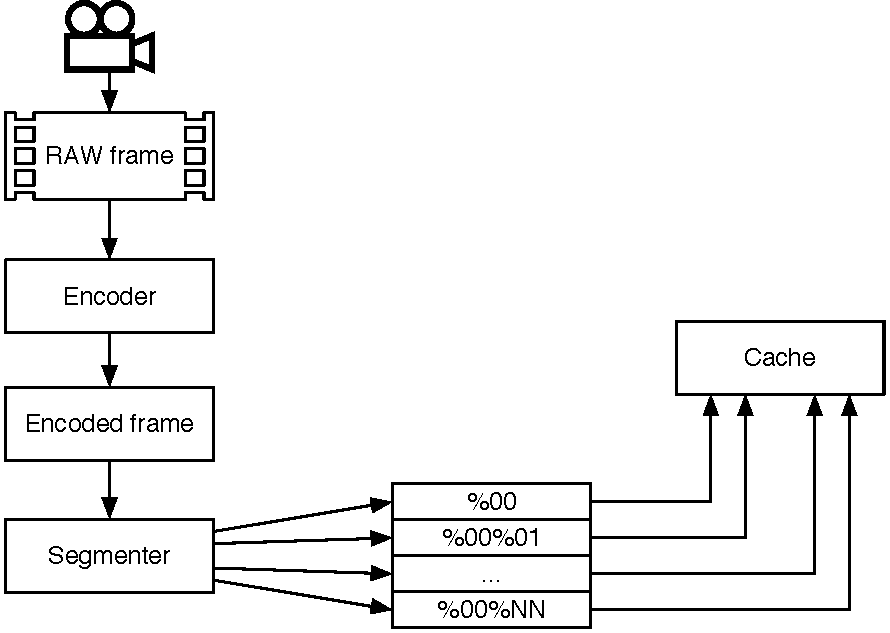
\includegraphics[width=0.4\textwidth]{producer}}\qquad
\subfigure[Consumer]{\label{fig:consumer}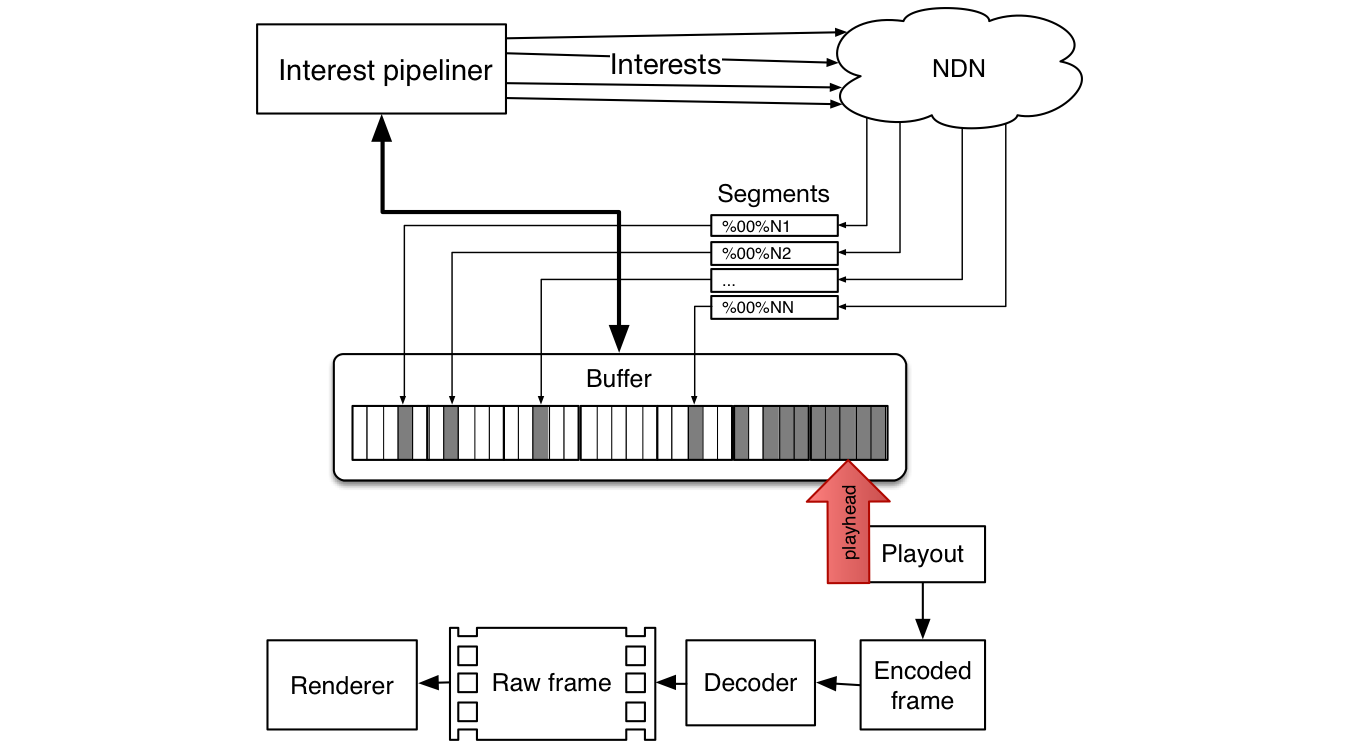
\includegraphics[width=0.4\textwidth]{consumer}}
\caption{\ndnrtcName{} producer and consumer operation.}
\end{figure}

There are two application roles in \ndnrtcName{}: producer and consumer.  In bidirectional communication, applications play both roles, but a variety of other multi-party and one-to-many scenarios can be achieved with the same abstraction.  The paradigm of real-time communication shifts from the sender-driven approach of the IP network, where the producer writes data to a destination host and the consumer reads it as it arrives, to a receiver-driven approach, in which the producer publishes data to network-connected storage at its own pace, while the consumer requests data as needed and manages the relationship between outgoing Interests, incoming data segments, and buffer fill. 
%%In the application????
% Redundant figure
%
%\begin{figure}[t!]
%\centering
%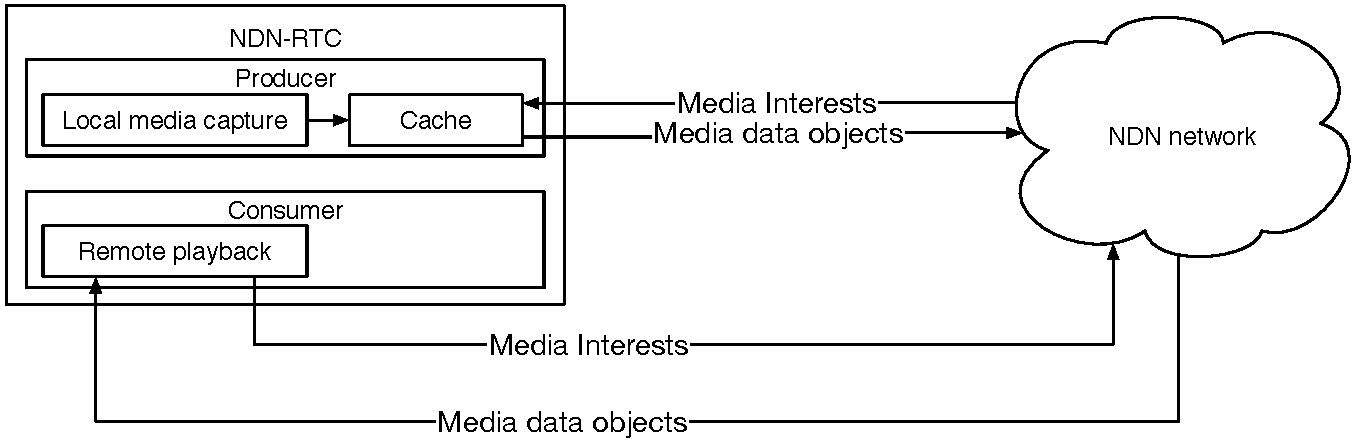
\includegraphics[width=0.5\textwidth]{architecture}
%\caption{RTC over NDN}
%\label{fig:arc}
%\end{figure}

% this paragraph describes figure which was considered redundant
%Figure \ref{fig:arc} presents a top-level overview of how \ndnrtcName{} works. Local media capture and cache belong to the producer. Media is stored in the cache which provides access to the data for all incoming Interests. Remote playback represents the consumer: issues Interests, prepares received media (assembles video frames from segments and re-orders them) and plays it back.

\subsection{Producer}
The producer's main tasks are to acquire video and audio data from media inputs, encode them, \textit{name them}, marshal the named data into network packets, sign the packets, and store them in an application-level cache\footnote{Currently, this cache is provided to the application by the NDN-CCL library.} that will asynchronously respond to incoming Interests. In this way, flow control responsibility shifts to the consumer, and scaling can be supported by network caches downstream rather than publishing infrastructure at the application level.  

%************************************************
\subsection{Namespace}

A primary design question is how the data should be named so it can be retrieved by the consumer with desired properties. The \ndnrtcName{} namespace defines names for media (segmented video frames and bundled audio samples), error correction data, and metadata, as shown in Figure~\ref{fig:namespace}.  As there is no direct consumer-producer communication, the namespace is designed to efficiently support the type of fetching operations performed by the consumer, as introduced in Section~\ref{sec:arch} and detailed in Section~\ref{sec:consumer}. 
%Besides that, the namespace should also reflect data specialization hierarchy - from general concepts in the root to more specialized entities towards the leaves. 

\subsubsection{Media} 

The \ndnrtcName{} producer abstracts the published media for a given source as a collection of \textit{media streams}. A media stream represents a flow of media data, such as video frames or audio samples, coming from a source--currently, an input device on the producer. (For now, names for streams are derived from their corresponding device information.) A typical publisher will publish several media streams simultaneously--e.g., a camera and a microphone, but also a separate stream for screenshots.  The data from a stream is encoded at one or more bitrates configured on the producer, so in the name hierarchy, each stream has children corresponding to different encoder instances called \textit{media threads}. Media threads allow the producer to, for example, provide the same media stream in several quality levels, such as low, medium and high quality, so that the consumer can choose the media thread suitable for its requirements and current network conditions.

%\begin{figure}[t!]
%\centering
%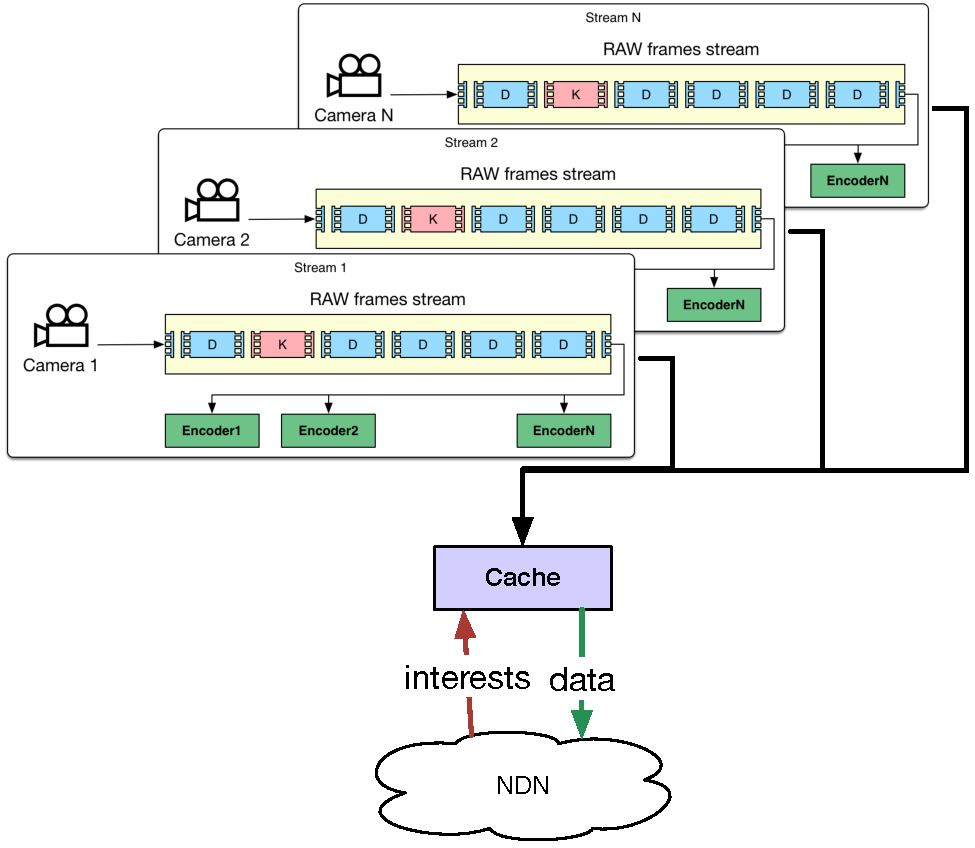
\includegraphics[width=0.5\textwidth]{streams-hierarchy}
%\caption{\ndnrtcName{} media streams hierarchy}
%\label{fig:stream-hierarchy}
%\end{figure}
\ndnrtcName{} packetizes the WebRTC video encoder output directly. Encoded media segments published under the hierarchical names described above, with video frames further separated into two namespaces per frame type, \texttt{delta} and \texttt{key}, each numbered sequentially and independently.  For reasons described in Section~\ref{sec:eval}, the namespace distinguishes in this way between two types of encoded video frames, key and delta frames. Key frames do not depend on any previous frames to be decoded. Delta frames are dependent on the previous frames (received after the last key frame), and cannot be decoded without significant visual artifacts if any of the key frames are missing. As needed, frame data is segmented with continuous sequence numbers per frame time.\footnote{For example, the average sizes of frames for 1000 kbps stream using VP8/VP9: key frames are $\approx$ 30KB, and delta frames are $\approx$ 3-7KB. Therefore, depending on the underlying transport's performance for delivering objects of this size, the producer may need to segment encoded frames into smaller chunks and name them in a way that makes reassembly straightforward. Based on our current observations of performance and the prevalence of UDP as a transport for the NDN testbed, \ndnrtcName{} currently packetizes media into segments that are less than the typical 1500 byte MTU.}

%%Encoded media segments published under the hierarchical names described above, with video frames further separated into two namespaces per frame type, \texttt{delta} and \texttt{key}, each numbered sequentially and independently. ---- This sentence needs to be reworded.

The next level in the tree separates data by type, either media or parity. Parity data for forward error correction, if the producer opts to publish it, can be used by a consumer to recover frames that miss one or more segments. 
%% What was motivation for separating FEC naming this way and not some other way? 
%% PG: i believe it's just implementation - having parity data named similar to media gives the advantage of using existing fetching/assembling algorithms on the consumer side
In the case of both parity and regular frames, the deepest level of the namespace defines individual data segments. These segments are numbered sequentially, and their names conform to NDN naming conventions \cite{ndnnaming}.

Audio streams are handled more simply, as their samples are much smaller than the maximum payload size, and there is no equivalent to the key/delta frame distinction in the audio codecs in use. All audio packets are published under the \texttt{delta} namespace. Multiple audio samples are bundled into one data packet, until the size of one data segment is reached, and published only after that.
%% How is audio/video sync maintained?? 
%% PG: there are timestamps included in metadata described in the next sections which are used for AV sync

\begin{figure}[t!]
\centering
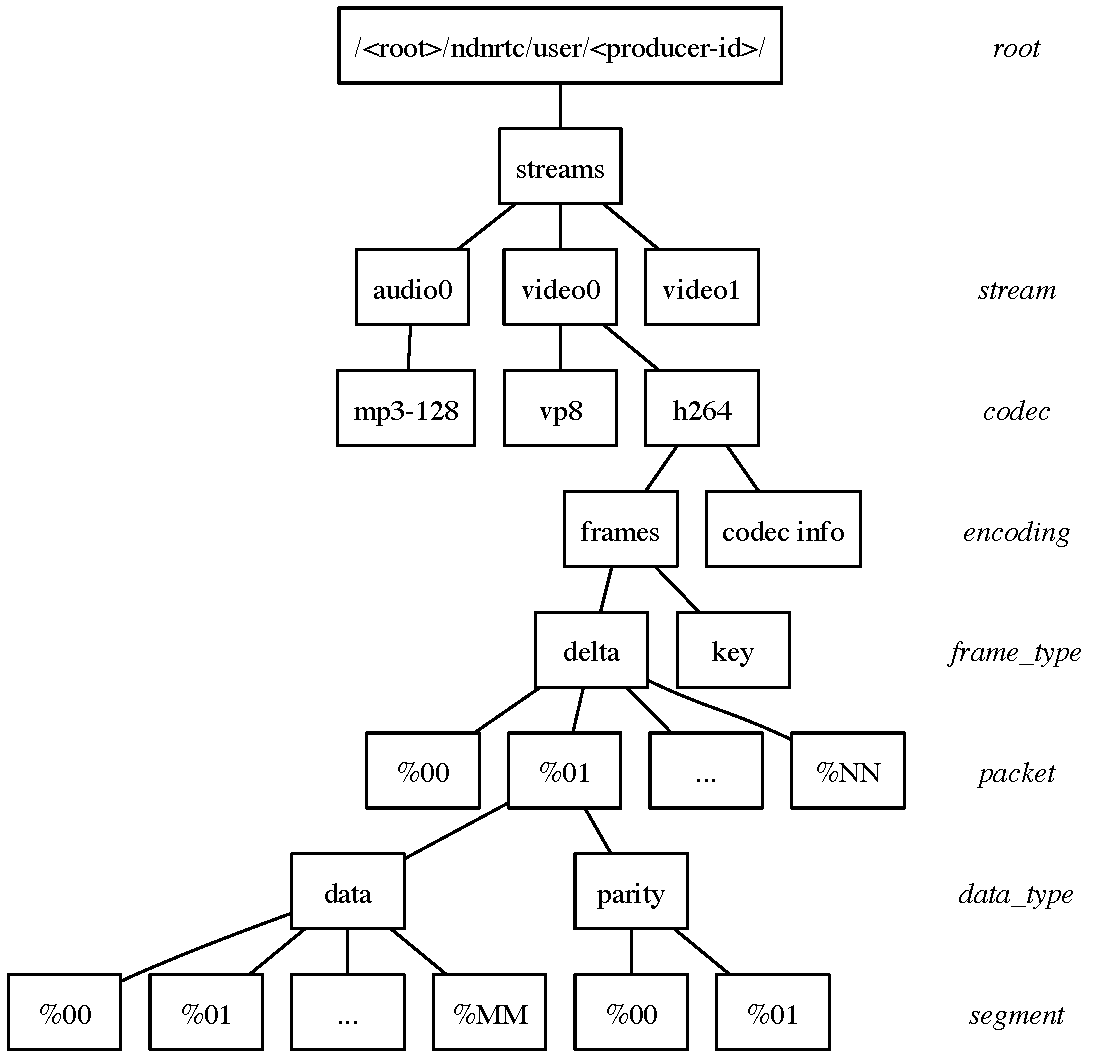
\includegraphics[width=0.45\textwidth]{namespace}
\caption{\ndnrtcName{} namespace}
\label{fig:namespace}
\end{figure}

\subsubsection{Metadata} 

\ndnrtcName{} uses both stream-level and packet-level metadata. Consumers need to know the producer's specific namespace structure in order to fetch data successfully. To save consumers from traversing the producer's namespace, the producer publishes meta-information about current streams under the \texttt{session info} at the rate of 1Hz. 
%% How often? PG: 1Hz
Thus, consumers can retrieve current information about the producer's publishing state.
%% state and "up-to-date" are ambigiuous here - what do they mean
%% PG: re-phrased a little bit. whenever producer adds/removes new streams, consumer will know about this by fetching session_info
Additionally, data names carry further metadata as part of each packet, which can be used by consumers regardless of which frame segment was received first. 
Four components are added at the end of every data segment name:
%% should really use texttt convention for names, I think
\small\begin{equation}
\texttt{\textit{seg\_name}/\textbf{num\_seg}/\textbf{playback\_pos}/\textbf{paired\_seq\#}/\textbf{num\_parity} \nonumber}
\end{equation}\normalsize
\begin{itemize}[label={}]
\item \texttt{num\_seg} - total number of segments for this frame;
\item \texttt{playback\_pos} - absolute playback position for current frame; this is different from the \textit{frame}, which is a sequence number for the frame in its domain (i.e. \texttt{key} or \texttt{delta});
\item \texttt{paired\_seq} - sequence number of the corresponding frame from other domain (i.e., for delta frames, it is the sequence number of the corresponding key frame required for decoding);
\item \texttt{num\_parity} - number of parity segments for the frame.
\end{itemize}
Metadata in the name, rather than in the packet, is expected to be useful for application components or services that may not need to understand or with to decode the packet payload. 
%%or with to decode the packet payload. This last part of the last sentence is not following the sentence.
%************************************************
\subsection{Data objects}
The producer generates signed data objects from input media streams and places them in an in-memory, application-level cache.  These objects contain stream data and metadata.

\subsubsection{Media stream}
Each media packet payload consists of two types of data -- a chunk from the media stream and metadata that describes it. Video stream data contains raw bytes received from the WebRTC library's video encoder, which represent the encoded frame. For audio, \ndnrtcName{} captures and encapsulates RTP and RTCP packets coming from the WebRTC audio processing pipeline, in order to obtain echo cancellation, gain control and other features, which are then fed into a similar pipeline on the consumer side for proper rendering and corrections.\footnote{This is an artifact of the current implementation to benefit from the full audio pipeline of WebRTC; features of these protocols are not used, would be eliminated in the future.}

\begin{figure}[t!]
\centering
\subfigure[Video frame segmentation.]{\label{fig:segment}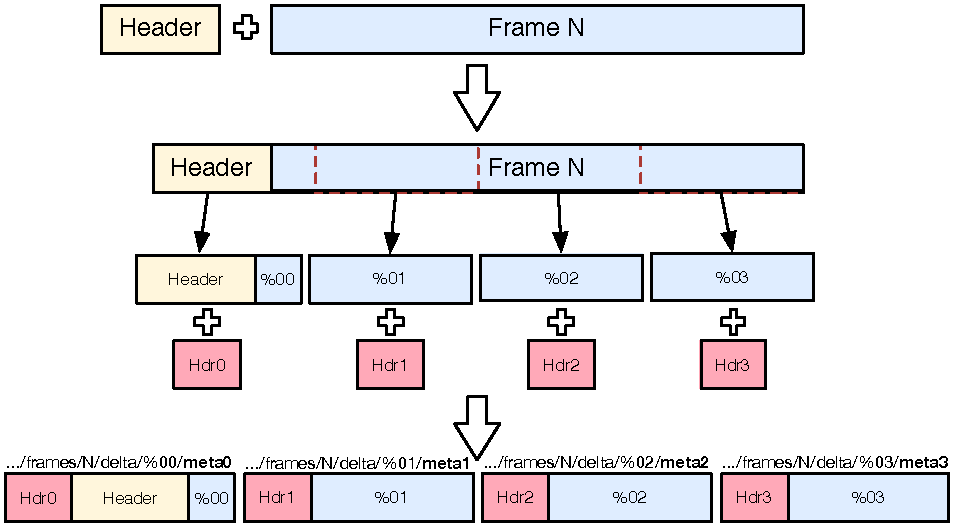
\includegraphics[width=0.5\textwidth]{segmentation}}
\subfigure[Audio sample bundling.]{\label{fig:audio-bundling}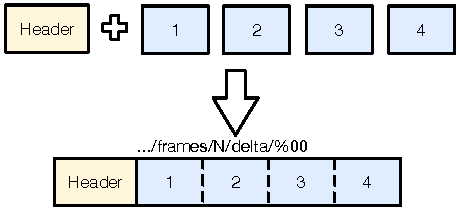
\includegraphics[width=0.3\textwidth]{audio-bundling}}
\caption{Segmentation and bundling}
\end{figure}

\subsubsection{Metadata}

The receiver-driven architecture of \ndnrtcName{} and our experimental approach's deliberate avoidance of explicit consumer-producer synchronization (to explore network scaling support) have suggested the importance of providing sufficient meta information from the producer. The most critical and potentially most useful for a variety of applications and services is provided in the namespace, as described above.  Other information is provided in the data objects themselves. Such separation is currently experimental and provides some benefits, e.g., quickly being able to retrieve the total number of segments in the frame without the need for content decoding or knowledge of the exact payload format.
%  You really should verify the name... so I took avoiding verification out
%

%%%%%%%% Need to explain why some metadata is in the name, and why some is in the payload!!! What type goes where? 
%% PG: I know =\ The truth is - it was experimental and, sort of, "transitional" after the news that finalBlockId is going to be deprecated. besides that, it's sometimes handy to just quickly retrieve data from the name rather to deal with the payload - verification, parsing, checking, etc... 

Packet-level metadata is applied to video as a header prepended to segment \#0 (see Figure \ref{fig:segment}). Each audio bundle (packet) is prepended by the same frame header, as seen in Figure \ref{fig:audio-bundling}. There are two header types: \textit{frame} and \textit{segment}. The frame header contains media-specific information (such as frame size), timestamp, current rate and Unix timestamp\footnote{Producer timestamp is \textit{not} required but can be used for calculating actual delay between NTP-synchronized producers and consumers)} (see Figure \ref{fig:data-struct}).

%%%% The following paragraph may be a little controversial
%%%% You should clarify whether consumers that do not issue the 
%%%% specific interest reported can really make use of it
%% PG: if nonce value does not bleong to the interest issued by consumer, this data does not make any sense for this consumer
Additionally, as an aid for experimentation and for optimizing two-way conversations, the segment header also carries the producer's observations of Interest arrival that can be used by consumers to hint fetching and playback choices.  The latter makes use of the Interest nonce value, and thus may not be as useful in larger multi-party calls. For this reason, we consider these primarily for debugging and experimental purposes at this time:
\begin{itemize} [label={}]
\item \textit{Interest nonce}: Nonce of the Interest which \textit{first} requested this particular segment. Example interpretations include the following:  1) Value belongs to an Interest issued previously: consumer received non-cached data requested by previously issued Interest; 2) Value is non-zero, but it does not belong to any of the previously issued Interests:  consumer received data requested by some other consumer; data may be cached.
\item \textit{Interest arrival timestamp}: Timestamp of the Interest arrival. Monitoring publisher arrival timestamps may give consumers information about how long it takes for Interests to reach the producer. This value is only valid when the nonce value belongs to one of a given consumer's Interests.
\item \textit{Generation delay}: Time interval in milliseconds between Interest arrival and segment publishing. A consumer can use this value in order to control the number of outstanding Interests. This value is again only valid when the nonce value belongs to one of the consumer's Interests.
\end{itemize}


%% The following paragraphs is relocated and was unclear

% This one seems to duplicate the above- 
%
%Such information (which could include Interests' nonce values, Interests' arrival timestamps and data generation delays), if added to the returned data segment, may help consumers evaluate relevant network performance, detect congestion, and assess whether incoming data is likely to be stale (delayed beyond the path delay). 

% This seems to either be future work, or on the consumer side.  It is
% unclear whey it was above
%
%Furthermore, keeping historical data on the consumer side may help Interest pipelining in the future. For instance, providing the average number of segments per frame type helps consumers estimate the number of required initial Interests to fetch upcoming frames. This helps keep frame fetching cycles minimal.


\begin{figure}[t!]
\centering
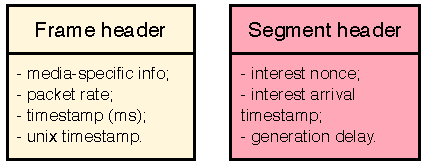
\includegraphics[width=0.3\textwidth]{data-struct}
\vspace{-4pt}
\caption{Frame and (experimental) segment headers.}
\label{fig:data-struct}
\end{figure}


%************************************************
\subsection{Consumer}
\label{sec:consumer}

While the data is published in the above scheme, in \ndnrtcName{}'s receiver-driven architecture, the consumer then aims to 1) choose the most appropriate media stream bandwidth from those provided by the producer (by monitoring network conditions); 2) fetch (and, if necessary, reassemble) media in the correct order for playback; 3) mitigate, as far as possible, the impact of network latency and packet drops on the viewer's quality of experience.  

%************************************************
\subsubsection{Interest pipelining and Data buffering}

The consumer implements Interest pipelining and data buffering, as shown in Figure \ref{fig:consumer}, to fetch and reassemble video and audio data while allowing for out-of-order arrival and interest reexpression. An asynchronous Interest pipeline issues Interests for individual segments. Independently, a frame buffer handles re-ordering of packets, and informs the pipeline of its status to prompt interest reexpression.
%%
%% Peter, you really should talk about how the buffer and pipeliner 
%% interact somewhere as this is really interest.
%%


%************************************************
\subsubsection{Frame fetching}

The consumer obtains the number of segments per frame from metadata in the received segment; however, to minimize latency, it should issue a pipeline of Interests simultaneously.  Therefore, at first, the consumer uses an estimate of the number of segments it must fetch for a given frame, issuing $M$ Interests, as illustrated in Figure \ref{fig:pull}. If Interests arrive too early, they will be held in the producer's PIT and stay there until the frame is captured and packetized. We call the delay between Interest arrival and availability of the media data the \textbf{generation delay}, $d_{gen}$. Conceptually, we wish to keep this interval low, to avoid accumulating outstanding Interests with short lifetimes, but we also do not wish to have Interests arrive after data is published, as this increases latency from the end-user's perspective.  Once the encoded frame is segmented into $N$ segments and published, Interests $0 - M$ are answered and the Data returns to the requestor(s). 

Upon receiving the first data segment, the consumer knows from the metadata the exact number of segments for the current frame, and issues $N - M$ more Interests for the missing segments, if any. These segments will be satisfied by data with no generation delay, as the frame has been published already by the producer. The time interval between receiving the very first segment and when the frame is fully assembled is represented by $d_{asm}$ and called \textbf{assembly time}. Note that for frames that are smaller than the estimate, some Interests may go unanswered; this is currently a tradeoff made to try to keep latency low for the frame as a whole. These Interests have low lifetimes, of about 300ms. 
 

\begin{figure}[t!]
\centering
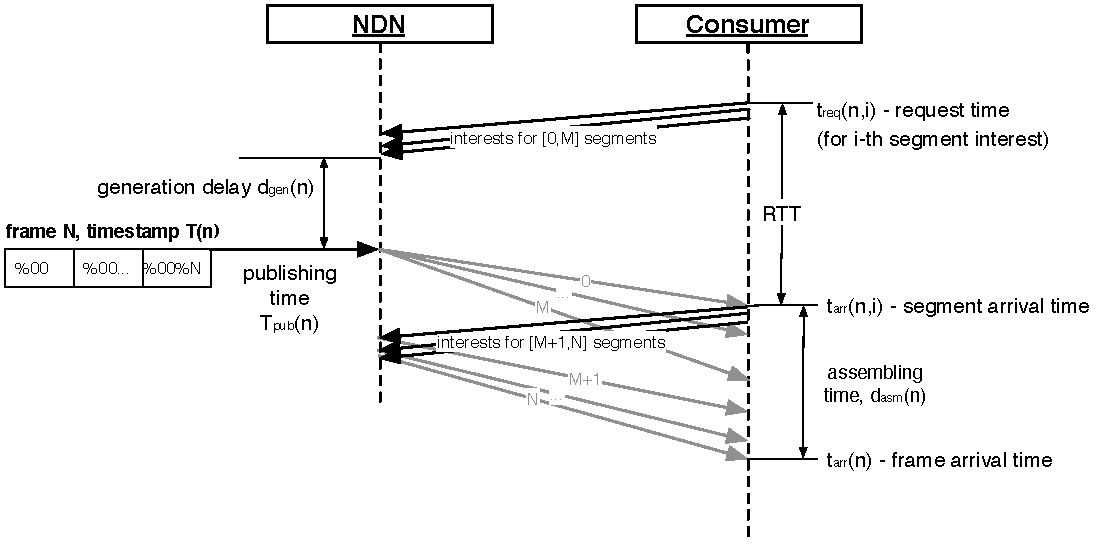
\includegraphics[width=0.5\textwidth]{frame-fetch}
\vspace{-18pt}
\caption{Fetching frame}
\label{fig:pull}
\end{figure}

Of course, additional round trips for requesting missing data segments increase overall frame assembly time and the possibility that the frame will be incomplete by the time it should be played back. This problem can be mitigated if the consumer is able to make more accurate estimates of the number of initial Interests. The latest versions of the library uses different namespaces for bitrates for key frames and delta frames, making it straightforward for the consumer to keep Interests outstanding for the next frame in each and to estimate the number of Interests needed per frame, as the average number of segments varies greatly for the two frame types. 
Additionally, the consumer tracks the average number of segments per frame type, adapting its estimates over time. A similar process is used for fetching audio, though for now, audio bundles are represented by just one segment.

\subsubsection{Buffering}

% Buffer:
% - re-ordering
% - added latency to mitigate network delays
% - extended defition:
% 	- pending frames
% 	- assembling frames
% - buffer-based retransmissions

As in sender-driven delivery, the consumer uses a ``jitter buffer" to manage out-of-order data arrivals and variations in network delay, and as a place to assemble segments into frames (see Figure \ref{fig:old-buf}). However, the role of such a buffer  has some NDN-specific aspects. In sender-driven video delivery, buffer slots can be allocated per segment using sequential numbering. 
A pull-based paradigm requires the consumer to request data by name explicitly, however, and organize it by frame as well as segment. Therefore, after expressing an Interest, the consumer ``knows" that new data is coming, and a named frame slot can be reserved in the buffer, though the number of segments is not known. Practically, this means that there will always be some number of reserved empty slots in the buffer. 

Thus, the \ndnrtcName{} jitter buffer's size is expressed in terms of two values measured in milliseconds: its \textit{playback size} is the playback duration in milliseconds of all complete ordered frames by the moment of retrieveing next frame from the buffer; its \textit{estimated size} is \textit{playback size} + \textit{number of reserved slots} $\times$ 1/\textit{producer rate} which reflects an estimated size of the buffer in case if all reserved slots have data.

The difference between estimated buffer size and playback size corresponds to the effective RTT, which we call $RTT^{\prime}$ (this cannot be smaller than the actual network RTT value). %Minimal $RTT^{\prime}$ value indicates that consumer receives the most recent data for the least amount of outstanding Interests. %% NOT CLEAR WHAT THIS MEANS 
%% PG: actually it's not entirely true - minimal RTT' could also mean that consumer is getting cached data...
Monitoring this value over times provides the consumer information on possible ``sync" status with the producer as will be described further below. %% HOW?. PG: described futher 
%For example, the consumer may use it during the fetching process, as will be discussed in the next section. 
%% Correct formatting for($RTT^{\prime}$)?

Another role played by the ``jitter buffer" is retransmission control. As shown in Figure \ref{fig:old-buf}, at some point inside the buffer ($J$ milliseconds from the buffer end) there is a checkpoint, where every frame is being checked for completeness. At the checkpoint, when incomplete frame can not be recovered using available parity data, Interests for the missing segments are re-issued. 

\subsubsection{Interest expression control}

%%  Probably want to cover all cases of interest rexpression here
%% - Prompted by timeouts in buffer
%% - To do the chasing

This section explores current mechanisms for Interest expression and re-expression in more detail.  A key challenge in a consumer-driven model for videoconferencing in a caching network appears to be how to ensure the consumer gets the latest data, without (per our design goal) resorting to direct producer-consumer communication.

To get fresh data, the consumer cannot rely on using such flags in the protocol as \textit{AnswerOriginKind} and \textit{RightMostChild}. The frame period for  streaming video is of the same order of magnitude of network round trip time, suggesting there is no guarantee that the data satisfying those flags received by a consumer will be the most recent one. Instead, it is necessary to use other indicators to ensure that the consumer is requesting and receiving the most up-to-date stream data possible given its (potentially evolving) network connectivity. 

Our current solution is to leverage the known segment publishing rate, which is available in stream-level metadata, and note that, under normal operation, old, cached samples are likely to be retrieved more quickly than new data.~\footnote{If the consumer is the \emph{only} consumer of the stream, its Interests will go directly to the publisher, which also yields the correct behavior. A more complex challenge, for further study, is when segments are inconsistently cached in different ways along the path(s) that Interests take.} We define the \textbf{interarrival delay} ($d_{arr}$) as the time between receipt of successive samples by a given consumer. 

The consumer expects that delays in the most recent samples follow the publishers' generation pattern, but cached data will follow the Interest expression's temporal pattern. Therefore, by monitoring inter-arrival delays of consecutive media samples and comparing them to the timing of its own Interest expression and the expected generation pattern, consumers can estimate data freshness (see Figure \ref{fig:inter-arrival}).

%%The following sentences really don't make much sense: To get fresh data, which can be cached but should not be the newest available for the consumer's path, the consumer cannot rely only on using such flags as \textit{AnswerOriginKind} and \textit{RightMostChild}. The high frequency nature of streaming data makes no guarantees that the data satisfying those flags received by a consumer will be the most recent one.


\begin{figure}[t!]
\centering

\subfigure[Bursty arrival of cached data, which reflects Interests expression pattern and indicates that the data is not the latest.]{\label{fig:cached}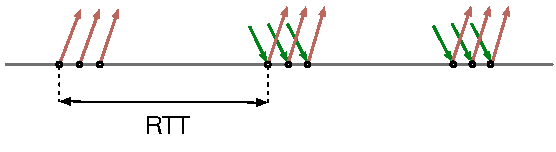
\includegraphics[width=0.4\textwidth]{arrival-cached}}\\
\subfigure[Periodic arrival of fresh data, reflects publishing pattern and sample rate.]{\label{fig:fresh}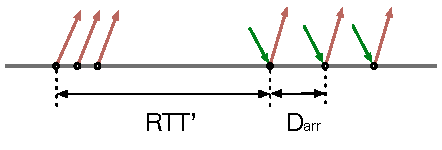
\includegraphics[width=0.35\textwidth]{arrival-fresh}}

\caption{Getting the latest data: arrival patterns for the cached and most recent data}
\label{fig:inter-arrival}
\end{figure}

\ndnrtcName{} interest expression is managed in two modes.  The \textit{bootstrapping mode} is active when a consumer first initiates data fetching and tries to exhaust cached data by changing the number of outstanding Interests. After the consumer has exhausted the cache, it switches into the \textit{playback mode}, described further below. 

During bootstrapping, the consumer ``chases" the producer and aims to exhaust network cache of historical (non-real time) segments. By increasing the number of outstanding Interests, the consumer ``pulls cached data" out of the network, unless the freshest data begin to arrive. 

In order to control Interest expression, the \ndnrtcName{} consumer tracks a quantity called ``\wConcept{}",  $\lambda$, which can be interpreted as how many outstanding Interests should be sent at the current time (see Figure \ref{fig:w-concept}). The consumer expresses new Interests when the demand is positive, i.e. $\lambda > 0$. For example, before the bootstrapping phase, the consumer initializes $\lambda$ with a value which reflects the consumer's estimate of how many Interests are needed in order to exhaust network cache and reach the most recent data. In playback, every time a new Interest is expressed, $\lambda$ is decremented, and when new data arrives, $\lambda$ is incremented, thus enabling the consumer to issue more Interests.\footnote{While inspired by the TCP congestion window, the \wConcept{}, as currently employed in \ndnrtcName{}, may play a different role in ICN networks, which we are exploring experimentally in this application.} 

\begin{figure}[t!]
\centering

\subfigure[``\wConcept{}" concept, $\lambda$]{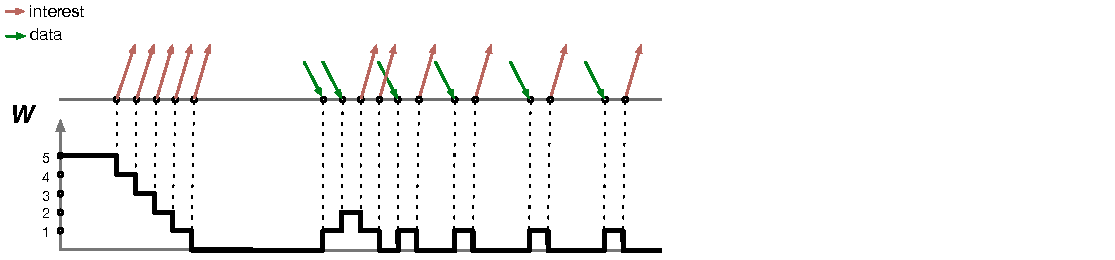
\includegraphics[width=0.35\textwidth]{w-concept}}
\subfigure[Interests bursting ($\lambda+3$)]{\label{fig:int-burst}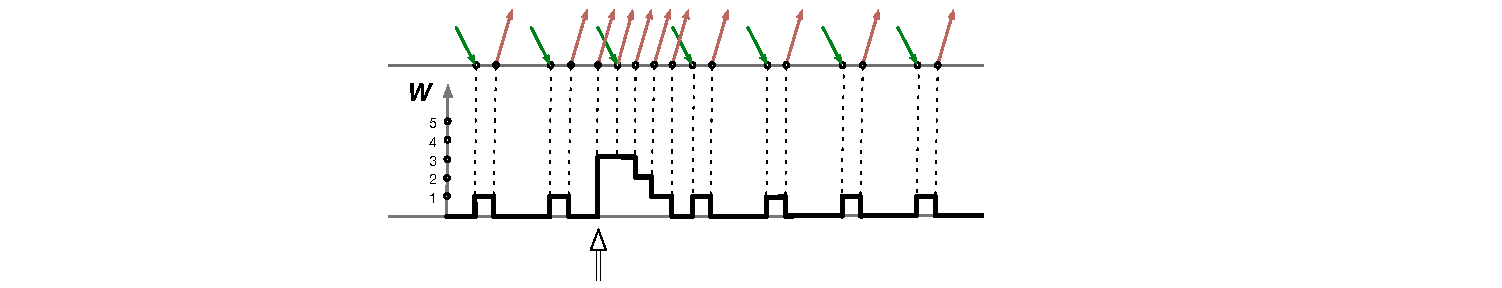
\includegraphics[width=0.35\textwidth]{int-burst}}
\subfigure[Interests withholding ($\lambda-3$)]{\label{fig:int-hold}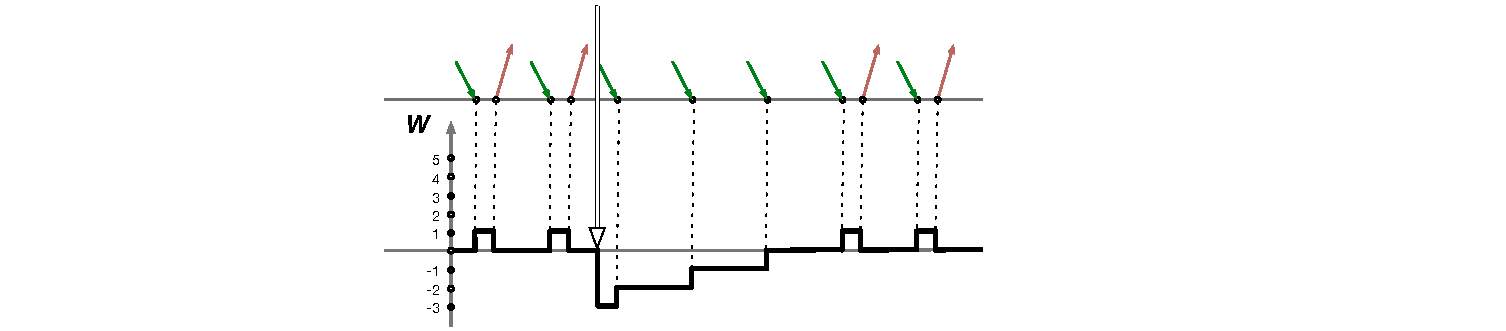
\includegraphics[width=0.35\textwidth]{int-hold}}

\caption{Managing Interest expression}
\label{fig:w-concept}
\end{figure}

\textbf{Bootstrapping.} In current design, there are two experimentally determined indicators that are used by the consumer to adjust $\lambda$: effective $RTT$ ($RTT^\prime$) and inter-arrival delay $d_{arr})$. As described above, at bootstrapping (and re-acquisition), the consumer interprets $d_{arr}$ stabilization around a relatively constant period, that means that consumer receives the freshest data available from the network. However, it does not necessarily mean that the consumer issues Interests efficiently. Figure \ref{fig:ws10} shows that even though the consumer has exhausted cache rather quickly, $RTT^\prime$ is three times larger than the actual $RTT$ for the network (100ms), which means that the majority of the issued Interests remain pending while waiting for the requested data to be produced.

The consumer makes several iterative attempts to adjust $\lambda$ during bootstrapping, which can be described as follows:
\begin{enumerate}
\item The consumer initializes \wConcept{} with $\lambda_d$, and initiates Interests expression.
\item If the consumer did not receive freshest data during allocated time\footnote{In the currently implementation, 1000ms.}, increase \wConcept{}: $\lambda=\lambda+0.5\lambda_d; \lambda_d = \lambda_d+0.5\lambda_d$.
\item \label{decrease-w} Whenever consumer receives freshest data (cache exhausted), decrease \wConcept{}: $\lambda=\lambda-0.5\lambda_d; \lambda_d = \lambda_-0.5\lambda_d$ and wait for either of the two possible outcomes:
a) $RTT^\prime$ decreases and the consumer still receives the freshest data -- go to step \ref{decrease-w};
b) the consumer starts to get cached data ($d_{arr}$ fluctuates greatly) -- restore previous value for $\lambda_d$, increase $\lambda$ accordingly and stop any further adjustments as the consumer has achieved sufficient synchronization with the producer.
\end{enumerate}

Note that bootstrapping begins with issuing an Interest with the enabled \textit{RightMostChild} selector, in \texttt{delta} namespace for audio and \texttt{key} namespace for video. The reason this process differs for video streams is that the consumer is not interested in fetching delta frames without having corresponding key frames for decoding. Once an initial data segment of a sample with number $S_{seed}$ has been received, the consumer initializes $\lambda$ with initial value $\lambda_d$ and asks for the next sample data $S_{seed}+1$ in the appropriate namespace. Upon receiving the first segments of sample $S_{seed}+1$, the consumer initiates the fetching process (described above) for all namespaces (\texttt{delta} and \texttt{key}, if available). The bootstrapping phase stops when the consumer finds the minimal value of $\lambda$ which still allows receiving the most recent data and the consumer switches to the playback mode.

% Listing \ref{lst:fetch-algo} shows pseudo-code for the bootstrapping phase.

% \begin{algorithm}
% \begin{algorithmic}

% \Function{Bootstrap}{Meta}

% \If {audio}
% 	\State $Nspc \gets DeltaNamespace$
% \Else
% 	\State $Nspc \gets KeyNamespace$
% \EndIf

% \State \Call{ExpressOne}{$RightMostChild$, $Nspc$}
% \Ensure Received data segment $dseed$
% \State $Sseed \gets$\Call{GetSeqNumber}{$dseed$}
% \State $NavgKey \gets$\Call{GetAvgSegNum}{$Meta$, $Key$}
% \State \Call{ExpressBulk}{$NavgKey$, $Sseed+1$, $Nspc$}
% \Ensure Received data segment $d$ for $Sseed+1$
% \State $J \gets$ \Call{GetDeltaNumber}{$d$}
% \State $NavgDelta \gets$\Call{GetAvgSegNum}{$Meta$, $delta$}
% \State $dW \gets N$
% \State $\lambda \gets DW$

% \While{$BootstrappingPhase$}

% \While{$\lambda > 0$}
% 	\State \Call{ExpressBulk}{$NavgDelta$, $J$, $delta$}
% 	\State $\lambda \gets W-1$
% 	\State $J \gets J+1$
% \EndWhile

% \If {received segment $dj$ for new sample}
% 	\State $\lambda \gets W+1$
% \EndIf

% \EndWhile

% \State \Call{Switch}{$FetchingPhase$}

% \EndFunction

% \end{algorithmic}

% \label{lst:fetch-algo}
% \caption{Bootstrap}
% \end{algorithm}

\textbf{Playback.}  During playback, $\lambda$ provides a manageable mechanism to speed up or slow down Interest expression, coupling the asynchronous interest expression mechanism with the status of the playback buffer. An increase in $\lambda$ value makes the consumer issue more Interests (Figure \ref{fig:int-burst}), whereas any decrease in $\lambda$ holds the consumer back from sending any new Interests (Figure \ref{fig:int-hold}). Larger values of $\lambda$ make the consumer reach a synchronized state with the producer more quickly. However, a larger value means a larger number of outstanding Interests and larger $RTT^\prime$ because of longer generation delays $d_{gen}$ for each media sample. By adjusting the value of $\lambda$ and observing inter-arrival delays $d_{arr}$, the consumer can find minimal $RTT^\prime$ value while still getting non-cached data, adapting towards a loose synchronization with the producer.

The consumer continues to observe $RTT^\prime$ and $d_{arr}$ in the playback mode. Whenever $d_{arr}$ indicates that no fresh data is being received, the consumer increases \wConcept{} and starts the adjusting process over again to find minimal $RTT^\prime$ for the new conditions. Such approach helps the consumers to adjust in cases when data may suddenly start to arrive from different network hub which introduces new network $RTT$.

\textbf{Interest batches.} Practically, for video, the consumer controls expression of ``batches" of Interests rather than individual Interests, because video frames are composed of several segments.  $\lambda$ is adjusted on a per-frame basis, rather than per-segment. 

\section{Implementation}
\label{sec:imp}
\ndnrtcName{} is implemented as a library written in C++, which is available at \url{https://github.com/remap/ndnrtc}. 
It provides a publisher API for publishing an arbitrary number of media streams (audio or video) and a consumer API with a callback for rendering decoded video frames in a host application. The OS X platform is currently supported; Linux build instructions will be added soon. 
The library distribution also comes with a simple console application which demonstrates the use of the \ndnrtcName{} library.

\ndnrtcName{} builds on functionality from several third-party libraries with which it is linked. NDN-CPP \cite{ndnccl} is used for NDN connectivity. The WebRTC framework \cite{webrtc} is used in two ways: 1) incorporation of the existing video codec; 2) full incorporation of the existing WebRTC audio pipeline, including echo cancellation. OpenFEC \cite{openfec} is used for forward error correction support. 

Some features were incorporated into the library based on our experience in this application.
% Should discuss memory content cache?
In most cases, consumers aim to express Interests for the data not yet produced, to be immediately satisfied when data is produced. The current NDN-CPP library provides a producer-side Memory Content Cache implementation into which data is published. However, this is only useful when data has been published and put in the cache before an Interest for this data has arrived. For the missing data, the Interest is forwarded to the producer application which stores it in the internal Pending Interests Table (PIT) unless requested data is ready. This functionality seems quite common for low-latency applications, and has now been incorporated into the NDN-CPP library implementation.

To demonstrate and evaluate the library, a desktop NDN videconferencing application, \ndnconName{}, \cite{ndncon} was implemented on top of \ndnrtcName{}. It provides a convenient user interface for publishing and fetching media streams, text chat, and organizing multi-party audio/video conferences. It was used, along with a command-line interface for the evaluation below.

\section{Evaluation \& Iterative refinement}
\label{sec:eval} 
During the course of \ndnrtcName{}'s initial development, there were several  design iterations that each introduced improvements in the overall quality of experience for the end user, as well as in application efficiency in terms of bandwidth and computation. Each iteration tackled problems that were revealed during tests. These motivated namespace, application packet format and other revisions, which are reflected in the design detailed above and described further in this section. 

\subsection{Video streaming performance}
A series of tests were conducted in order to assess bandwidth usage and perceived quality compared to Skype video calls. Each test was comprised of six runs of two-person, five-minute conference talks using \ndnconName{}, the graphical conferencing application built on top of \ndnrtcName{}: a) three runs of audio+video with low, medium and high video bandwidths settings (0.5, 0.7 and 1.5 Mbit/s accordingly); b) one run of audio-only conference; c) one run of Skype audio+video conference; d) one run of Skype audio-only conference. Tests were conducted across the existing NDN testbed, between the UCLA REMAP hub and six other hubs.  These tests covered both one-hop and multi-hop (with several intermediate hubs) paths. 

% Obvious - 
%Actual average bitrates turned out to be slightly higher than pre-configured video streams -- 0.7, 0.9 and 1.8 Mbit/s for low, medium and high bandwidths respectively-- which can be explained by NDN packet overhead which is approximately 280-330 bytes and accounts for $\approx$30\% of the segment size (1000 bytes). 

Figure \ref{fig:tests-skype} shows overall bitrate usage results. Whereas Skype has adapted to use link capacity between peers, and delivered higher bitrate videos, NdnCon did not adjust to the current network conditions which make adaptive rate control features highly desirable as future work. Early in these tests, audio sample bundling was quickly introduced in \ndnrtcName{} to reduce audio bandwidth (and the number of Interests on the consumer side), making it comparable to Skype audio bandwidths.

% Obvious - 
%
%Having such large overhead makes transferring audio samples in separate segments highly inefficient. 

\begin{figure}[t!]
\centering
\begin{tiny}
\def\svgwidth{0.5\textwidth}\input{tests-skype.pdf_tex}
\end{tiny}
\vspace{-18pt}
\caption{2-peer conference tests compared to Skype}
\label{fig:tests-skype}
\end{figure}

%The overall user experience for these 2-person conferences was subjectively assessed as being higher than average - 3 points on a scale from 0 to 5 (Skype calls were taken as 5-point user experiences).
%%% I would not include this. 

The results of such testing influenced iterative updates to the design, two of which are described below. 

\textbf{Separation of key and delta frame namespaces.} Video streaming performance in early versions of \ndnrtcName{} suffered from video ``hiccups", even when being tested on trivial one-hop topologies. The cause of this problem turned out to be an inefficient frame fetching process.
 In early \ndnrtcName{} versions, the difference in size, and thus segments, of key frames and delta frames was not reflected in the producer's namespace and consumers were forced to issue equal number of initial Interests ($M$ on Figure \ref{fig:pull}) regardless of the frame type. This resulted in additional round trips of missing Interests and, consequently, larger assembling times ($d_{asm}$) for key frames that resulted in missed playout deadlines. Having a separate namespace for key frames enables consumers to maintain separate Interest pipelines per frame type and collect historical data on the average number of Interests required to retrieve one frame of each type in one round trip. 

%Increased assembling time quite often caused skipping incomplete key frames, as they were not assembled by the time they should have been played out. Eventually, all the subsequent delta frames were skipped as well, which degraded the overall video streaming experience by introducing the video ``hiccup" effect. 
%%which made consumer to pipeline equal number of initial Interests--- this makes little sense to me, if any.
%% PG: tried to rephrase...

%\subsection{Quality of experience}
% PG: moved figure to the previous section


\subsection{Consumer-Producer synchronization}

\begin{figure}[t!]
\centering
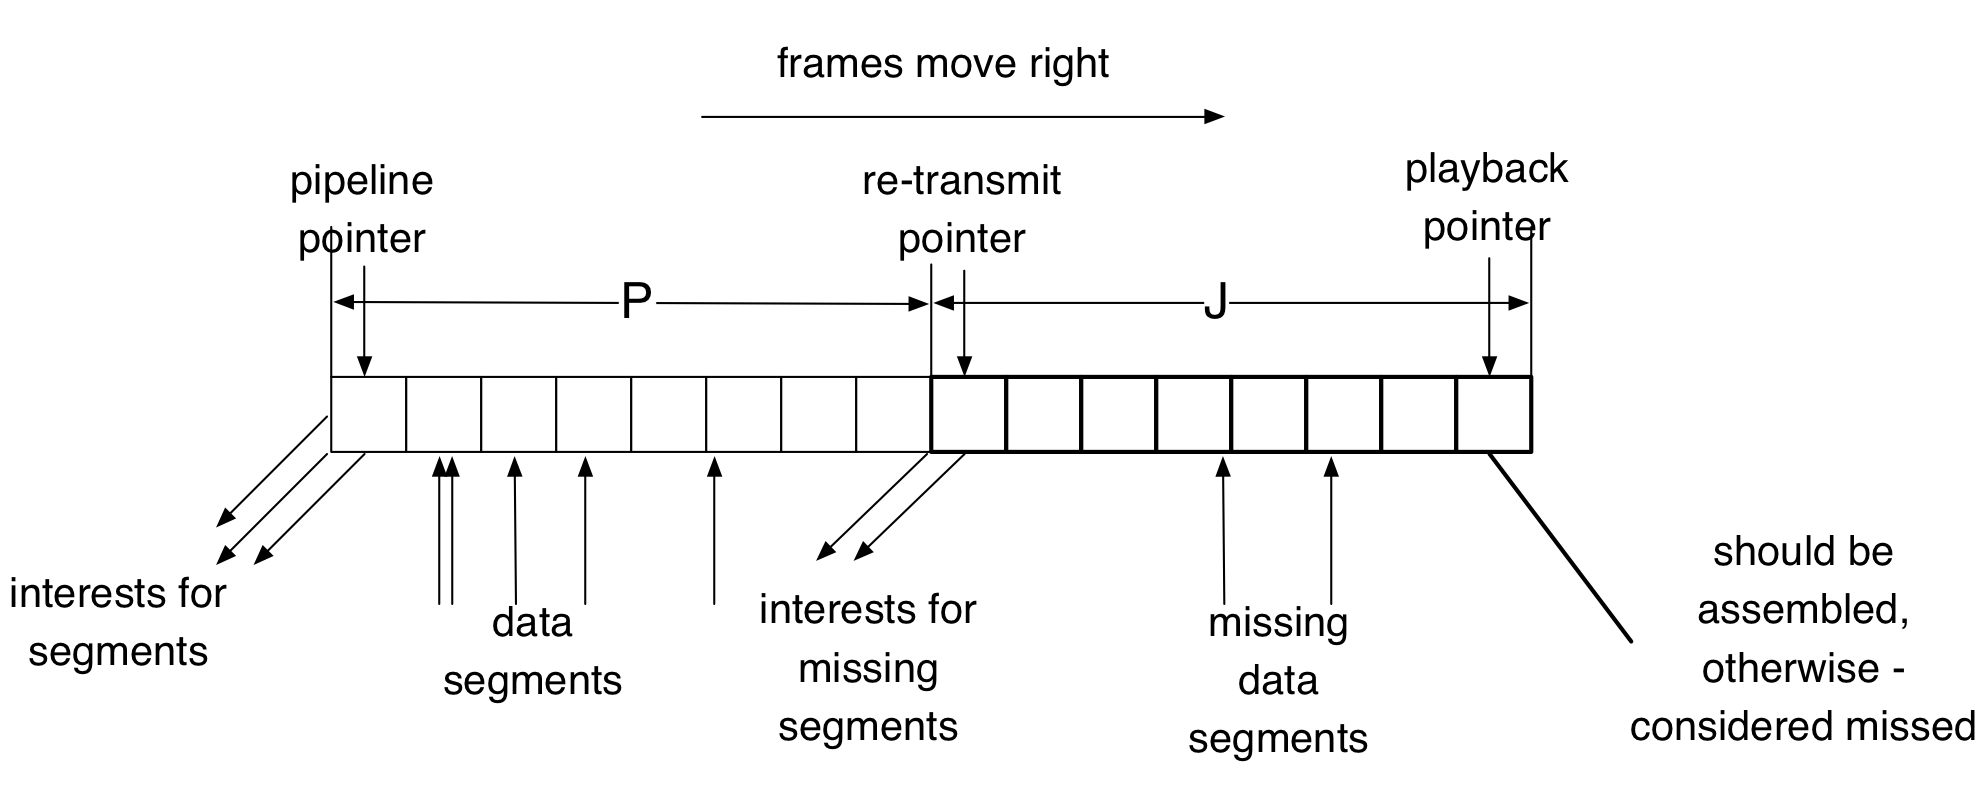
\includegraphics[width=0.5\textwidth]{buffer}
\caption{Frame buffer}
\label{fig:old-buf}
\end{figure}


%%% -- This figure is not cited!

%\begin{figure}[t!]
%\centering
%
%\subfigure[$d_{gen} \approx 600ms$ resulted in 50\% retranmissions]{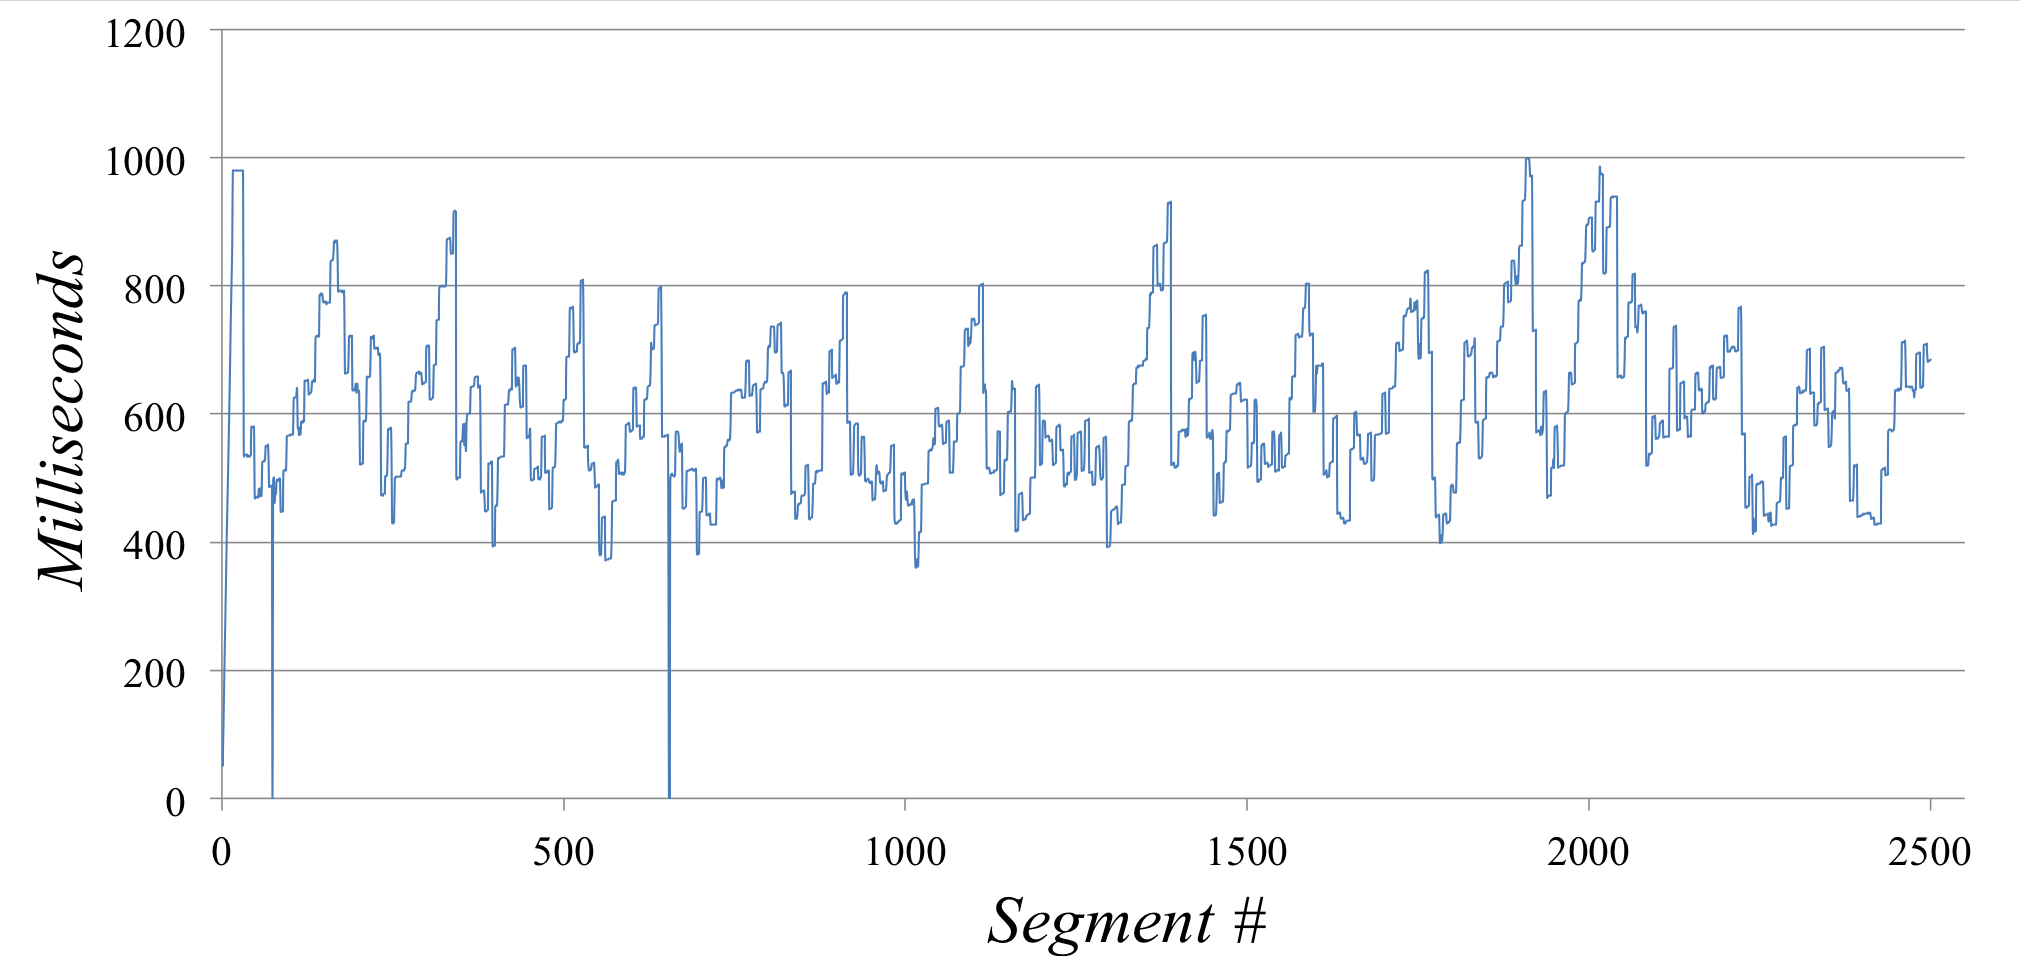
\includegraphics[width=0.4\textwidth]{dgen-bad}}
%\subfigure[$d_{gen} \approx 310ms$ - no redundant retransmissions]{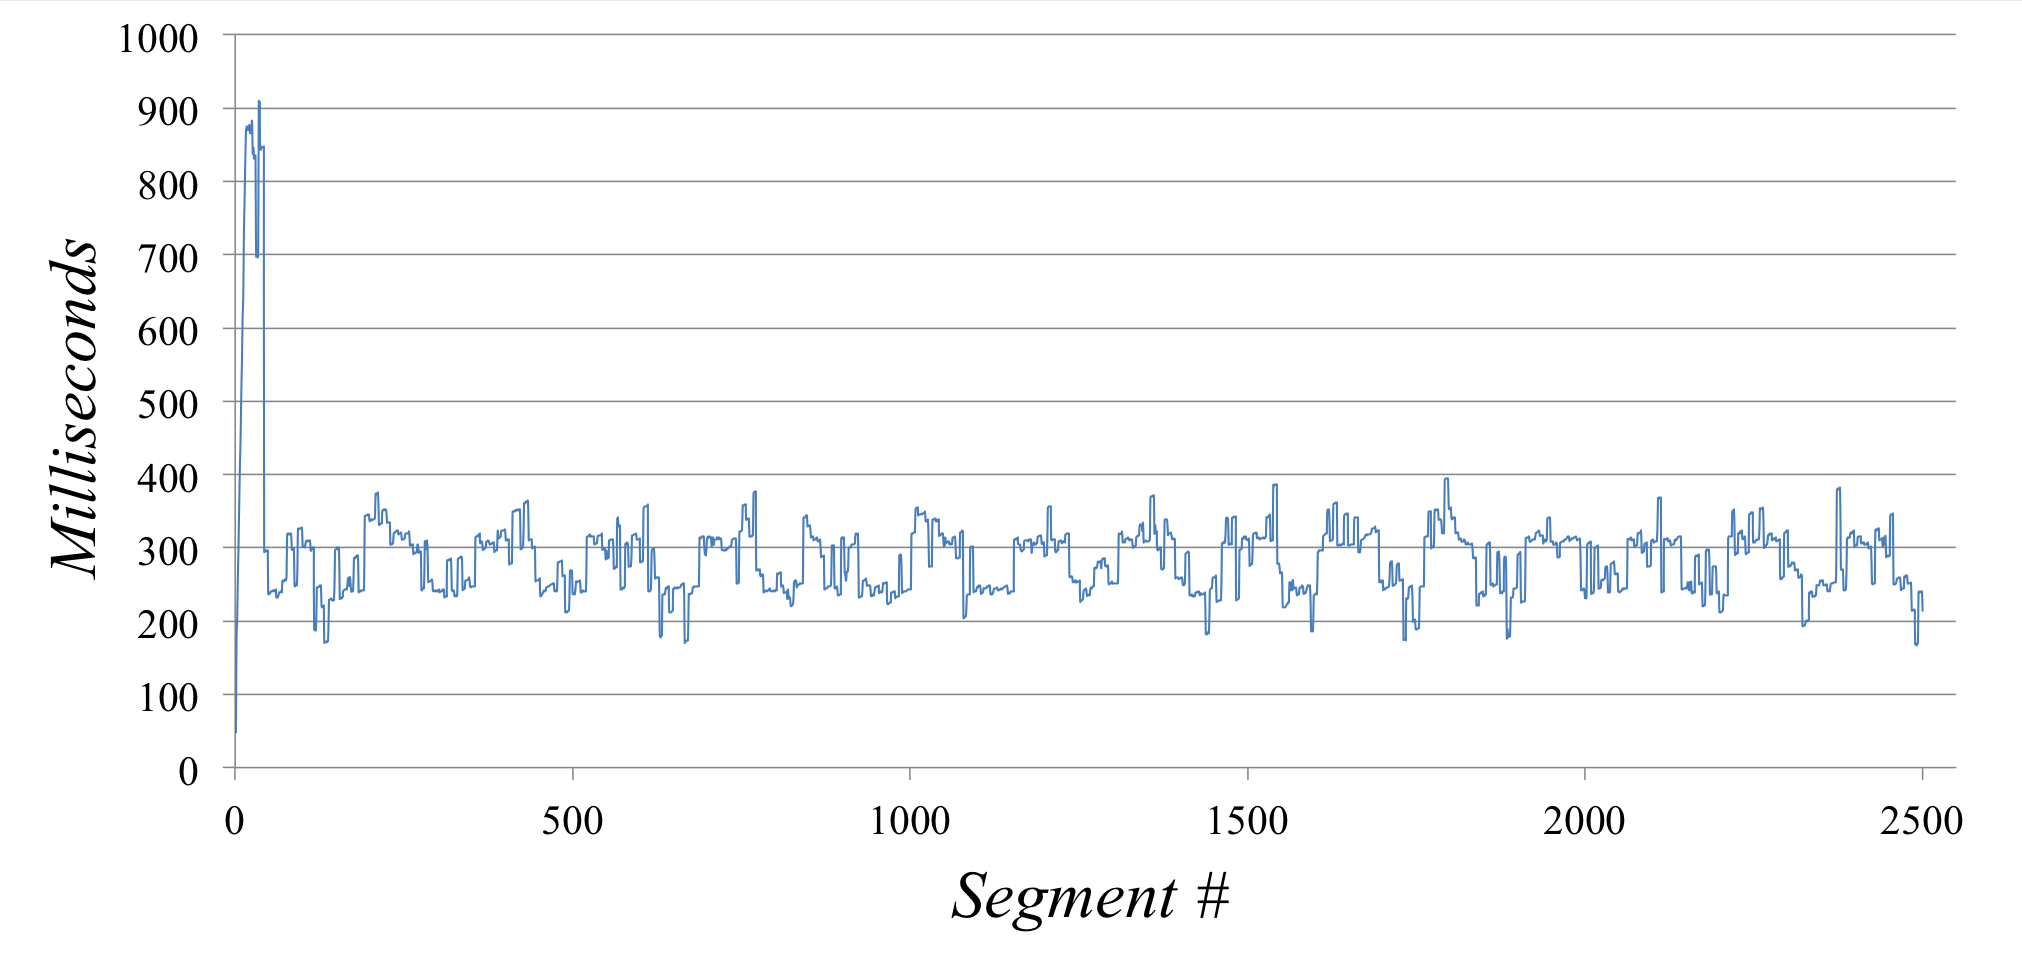
\includegraphics[width=0.4\textwidth]{dgen-decent}}
%
%\caption{Two separate runs of earlier library version on similar topology (one-hop): random results for data generation delay $d_{gen}$ due to poor consumer-producer synchronization.}
%\label{fig:dgen}
%\end{figure}

\textbf{Bootstrap behavior.} In initial library versions based on the approach taken in NDNVideo, the consumer ``chased" the producer's time-series data by exhausting cached data via issuing a large number of outstanding Interests. However, there was no mechanism for the consumer to figure out when to issue those Interests and whether Interest expression should be postponed in order to reduce timeouts. For two similar test runs (one-hop topology), the number of timed out Interests and re-transmissions varied greatly (either $\approx$1\% or $\approx$50\%). One was due to an incorrect consumer's synchronization with the producer; Interests were issued too early, so they timed out before any data had been produced. This problem was addressed by increasing the Interests' lifetime. 

However, for previous library versions, the mechanism for buffering (see Figure \ref{fig:old-buf}) dictated the Interests' lifetime. In fact, in order to maintain the re-transmission checkpoint, all Interests entering the buffer had a lifetime equal to half of the current buffer size. This approach resulted in unavoidable Interest timeouts, in the cases when the consumer issued Interests far too early, before the actual data was produced.  This was further complicated by forwarding strategies in NFD that did not handle consumer-initiated retransmission over short periods. 

For the current version of the library, the re-transmission checkpoint is placed at a time estimated to be the effective $RTT$ from the end of the buffer ($J=RTT$ on the Figure \ref{fig:old-buf}). This, together with an updated NFD re-transmission strategy \cite{nfd-rtx-release}, allows for larger Interests' lifetimes.



%%In the second sentence above, I changed it to until, but it was initially unless.

\begin{figure}[t!]
\centering
%\captionsetup[subfigure]{aboveskip=-1pt,belowskip=-2pt}
\begin{scriptsize}
\subfigure[$\lambda=10$: short chasing, larger $RTT^\prime$]{\label{fig:ws10}\def\svgwidth{0.48\textwidth}\input{w10.pdf_tex}}
\subfigure[$\lambda=4$: longer chasing, smaller $RTT^\prime$]{\label{fig:ws4}\def\svgwidth{0.48\textwidth}\input{w4.pdf_tex}}
\subfigure[$\lambda=3$: consumer can't exhasut cache, $RTT^\prime = RTT$]{\label{fig:ws3}\def\svgwidth{0.48\textwidth}\input{w3.pdf_tex}}
\end{scriptsize}
\caption{Larger $\lambda$ decreases ``chasing" phase, but increases $RTT^\prime$ for the same network configuration ($RTT\approx100ms$)}
\label{fig:ws}
\end{figure}

Moreover, the problem described above can not occur if the consumer knows that it is issuing Interests too early. The chasing algorithm in older library versions was exhausting the network cache too aggressively; Interests were issued constantly until they filled up the buffer.  With the introduction of the $\lambda$ concept, the consumer has more useful control of the Interest expression. Figure \ref{fig:ws} shows how a larger value of $\lambda$ helps to exhaust the cache more quickly. The number of outstanding Interests is controlled by a consumer and directly influences how fast consumer can ``chase" the producer. Thus, the consumer can control the ``agressiveness" of cache exhaustion.
%% PG: removed these sentences as they duplicate "Interest expression control" section
%The $\lambda$ concept allows a ``lazy" start for the consumer. By specifying a smaller $\lambda$, the consumer issues less Interests. Further, the consumer observes cache exhaustion by monitoring $d_{arr}$ and, if the cache has not been exhausted during allocated time, the consumer may increase the value of $\lambda$ in order to express more Interests. Similarly, the consumer may opt to decrease $\lambda$ in cases where the original value resulted in behaviour that is too aggressive.

%\subsection{Test setup} 

%Include testbed topologies used, collaboration with WUSTL

%- one-hop
%- multiple-hops
%- many-to-many conferencing

%\subsection{Quality of experience} 

%How was the end-user quality of experience by the time the paper was written
%What kinds of things did you add to support it. 

\subsection{Multi-party use}

\begin{figure}[t!]
\centering

\subfigure[NDN testbed utilization during biweekly NDN seminar using \ndnconName{} for simulcast.]{\label{fig:one-to-many}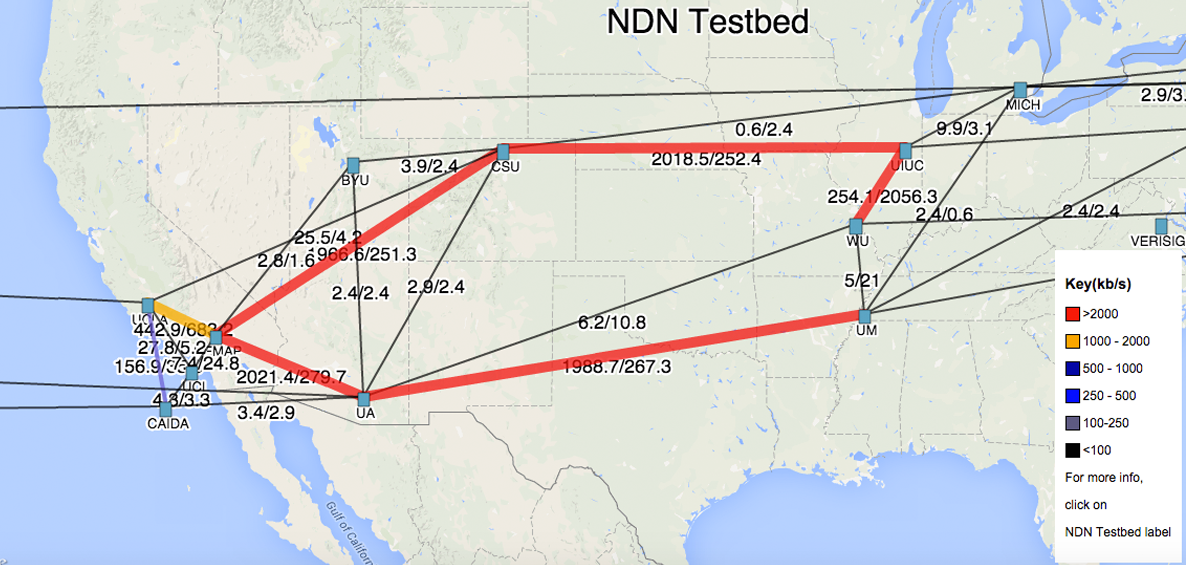
\includegraphics[width=0.5\textwidth]{confbridge}}
\subfigure[NDN testbed utilization during 4-peer call between UCLA, REMAP, WUSTL and CAIDA hubs.]{\label{fig:many-to-many}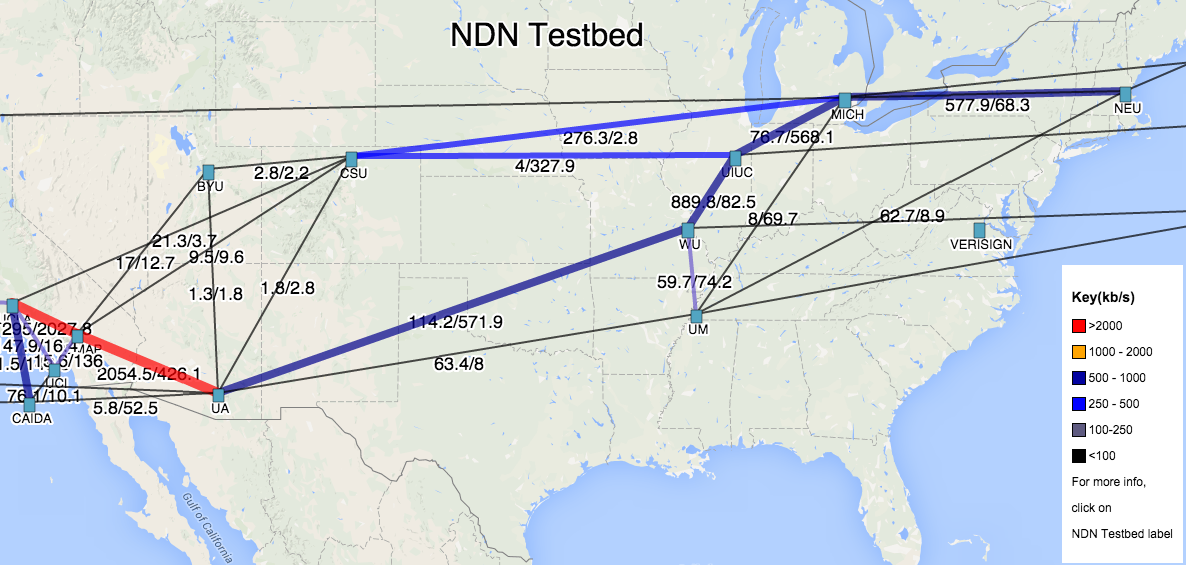
\includegraphics[width=0.5\textwidth]{4peer}}

\caption{NDN testbed utilization during one-to-many and many-to-many scenarios.}
\label{fig:testbed-utilization}
\end{figure}

Initial attempts to deploy the \ndnconName{} conferencing application were made in early 2015. \ndnconName{} was used to stream an NDN seminar over the existing NDN testbed. An audio/video bridge was set up using third-party tools, such as Soundflower and CamTwist Studio, allowing captured screen and audio feeds from existing IP-based conferencing tools to be simulcast. Figure \ref{fig:one-to-many} shows an example of instantaneous NDN testbed utilization during the one-hour conference call. It is estimated that media streams were consumed by five to eight people. Overall quality was satisfying, as reported by users.

Other tests of multi-party conferencing ability included four peers, each publishing three video streams and one audio stream and fetching one video and one audio stream from each of the other participants. Participants were distributed across four NDN testbed hubs - UCLA, REMAP, CAIDA and WUSTL (Figure \ref{fig:many-to-many}). These results were also generally satisfying. However, for one user, audio cutoffs occurred more often than for the other participants. The root causes of this have yet to be found. Many-to-many test scenarios are complex, and will be included in future work.
%%UCLA and REMAP? Or is there some clarification needed here?
%% PG: these are actually NDN testbed hubs, I've edited text

\section{Conclusion and Future Work}
\label{sec:conclusion}

\begin{figure}[t!]
\centering
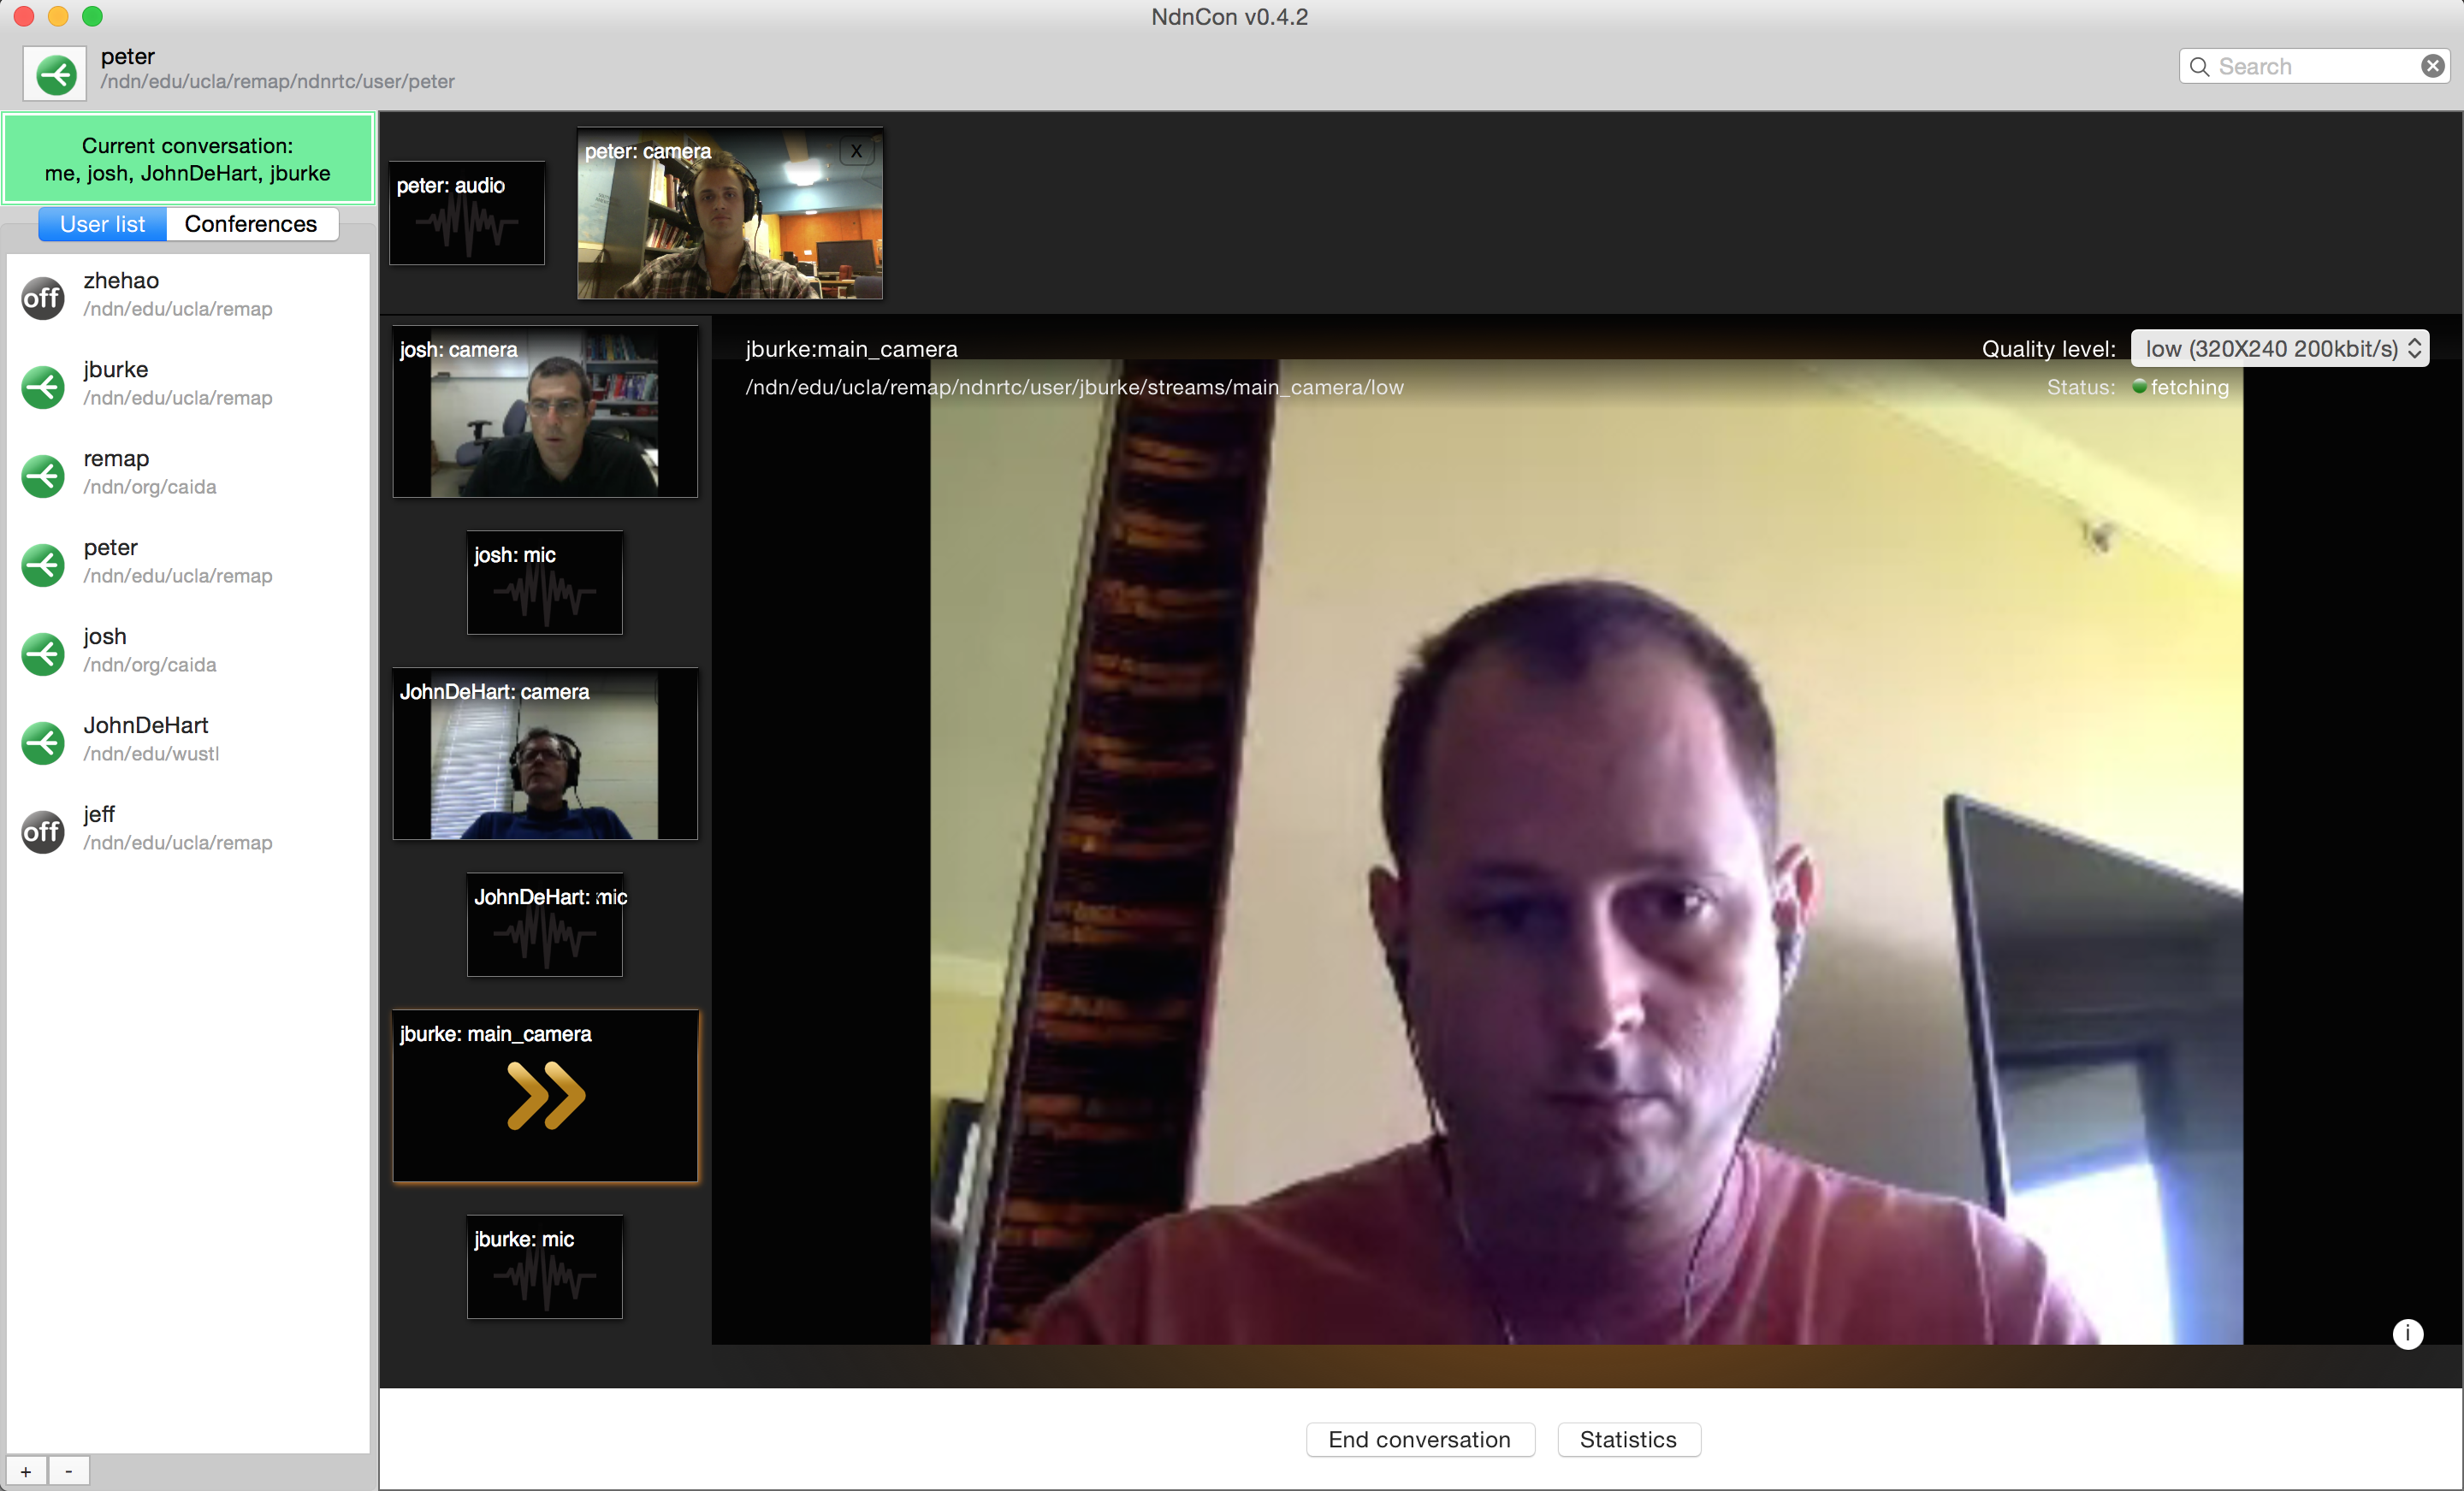
\includegraphics[width=0.3\textwidth]{ndncon}
\caption{\ndnconName{} screenshot.}
\label{fig:ndncon}
\end{figure}

%% TODO: Conclusion

This paper presents the design, implementation, and initial experimental evaluation of \ndnrtcName{}, a low-latency videoconferencing library built on Named Data Networking.   Our approach to this project has been experimentally driven so far, and has generated a functional low-latency streaming tool that we can now use a platform for exploring important design challenges in real-time media over NDN.  This is a rich area, and some of the future work that we have identified includes: 
\begin{itemize}[label={}]

\item \textbf{Adaptive rate control.} In the current design, the producer can choose to publish the same video stream at different bitrates, thus requiring the consuming user to manually select the best stream but laying the groundwork for adaptive rate control as a near-term effort. Such work will need to determine if monitoring of $d_arr$ and other approaches described above can address challenges of such adaptation over ICN, as suggested in papers such as \cite{posch2014client}.

\item \textbf{Congestion control.} Congestion control algorithms and their impact on the receiver-driven design of \ndnrtcName{} are an open challenge that requires collaboration between application developers and architecture researchers. 

\item \textbf{Audio prioritization.}  For quality of experience in typical audio/videoconferencing applications, audio should be prioritized over video.  This can be done at the application level, and we may provide such support in the future. % Others on the NDN team have proposed the notion of one-hop priority that would provide architecture support for relative prioritization of interests.

\item \textbf{Scalable video coding.} A more efficient way to relieve the producer from having to publish multiple copies of the same content at different bandwidths may be to use scalable video coding. By reflecting SVC layers in the namespace, the consumer will have more freedom for adapting media streams to the current network. Just as with audio, the SVC base layer may need to be prioritized. 

\item \textbf{Encryption-based access control.} The current \ndnrtcName{} design supports basic content signing and verification. However, a prominent requirement of many types of videoconferencing is confidentiality, which we expect can be supported through encryption-based access control.  While it may appear that encryption could limit the gains offered by caching, recent work exploring that application of advanced cryptographic techniques such as attribute-based encryption to multimedia in ICN \cite{papanis2014use} suggest interesting new directions for balancing benefits of ICN with security requirements. 
\end{itemize}
%\item \textbf{Conference management} 
%Work on ndncon. unknown but verified publishers trust; 
%\end{itemize}
%%signatures consistency checks for successive media packets 
%% need to add the above before publication %%;  


\section{Acknowledgements}
\label{sec:Acknowledgements}
This project was partially supported by the National Science Foundation (award CNS-1345318 and others) and a grant from Cisco. The authors thank Lixia Zhang, Van Jacobson, and David Oran, as well as Eiichi Muramoto, Takahiro Yoneda, and Ryota Ohnishi, for their input and feedback. John DeHart, Josh Polterock, Jeff Thompson, Zhehao Wang and others on the NDN team provided invaluable testing of \ndnconName{}.  The initial forward error correction approach in \ndnrtcName{} was by Daisuke Ando. 

\bibliographystyle{abbrv}
{\small
\bibliography{bibliography}
}

\end{document}